%%%%%%%%%%%%%%%%%%%%%%%%%%%%%%%%%%%%%%%%%%%%%%%%%%%%%%%%%%%%%%%%%%%%%%%%%
%                                                                       %
% ustthesis_test.tex: A template file for usage with ustthesis.cls      %
%                                                                       %
%%%%%%%%%%%%%%%%%%%%%%%%%%%%%%%%%%%%%%%%%%%%%%%%%%%%%%%%%%%%%%%%%%%%%%%%%

\documentclass{ustthesis}

% \usepackage{latexsym}
    % Use the "latexsym" package when encountering the following error:
    %   ! LaTeX Error: Command \??? not provided in base LaTeX2e.
% \usepackage{epsf}
    % Use the "epsf" package for including EPS files.

%%%%%%%%%%%%%%%%%%%%%%%%%%%%%%%%%%%%%%%%%%%%%%%%%%%%%%%%%%%%%%%%%%%%%%%%%
%                                                                       %
% Preambles. DO NOT ERASE THEM. Change to suite your particular purpose.%
%                                                                       %
%%%%%%%%%%%%%%%%%%%%%%%%%%%%%%%%%%%%%%%%%%%%%%%%%%%%%%%%%%%%%%%%%%%%%%%%%

\usepackage{enumitem}
\usepackage{times} %
\usepackage{helvet} %
\usepackage{courier} %
\usepackage{multirow} %
\usepackage{epsfig} %
\usepackage{verbatim} %
\usepackage{xcolor}
\usepackage{amsmath}
\usepackage{amssymb}
\usepackage{graphicx}
\usepackage[linesnumbered,ruled,vlined]{algorithm2e}
\usepackage{subfigure}
\usepackage{epsfig}
\usepackage{listings}
\usepackage[a4paper,top=2.5cm,bottom=2.5cm,left=2.5cm,right=2.5cm]{geometry}
\usepackage{cases}
\usepackage{url}
\usepackage{algorithmic}
\lstset{ %
  backgroundcolor=\color{white},   % choose the background color; you must add \usepackage{color} or \usepackage{xcolor}
  basicstyle=\footnotesize,        % the size of the fonts that are used for the code
  breakatwhitespace=false,         % sets if automatic breaks should only happen at whitespace
  breaklines=true,                 % sets automatic line breaking
  captionpos=b,                    % sets the caption-position to bottom
  %commentstyle=\color{mygreen},    % comment style
  deletekeywords={...},            % if you want to delete keywords from the given language
  escapeinside={\%*}{*)},          % if you want to add LaTeX within your code
  extendedchars=true,              % lets you use non-ASCII characters; for 8-bits encodings only, does not work with UTF-8
  frame=single,                    % adds a frame around the code
  keepspaces=true,                 % keeps spaces in text, useful for keeping indentation of code (possibly needs columns=flexible)
  keywordstyle=\color{blue},       % keyword style
  language=Octave,                 % the language of the code
  morekeywords={*,...},            % if you want to add more keywords to the set
  %numbers=left,                    % where to put the line-numbers; possible values are (none, left, right)
  %numbersep=5pt,                   % how far the line-numbers are from the code
  %numberstyle=\tiny\color{mygray}, % the style that is used for the line-numbers
  rulecolor=\color{black},         % if not set, the frame-color may be changed on line-breaks within not-black text (e.g. comments (green here))
  showspaces=false,                % show spaces everywhere adding particular underscores; it overrides 'showstringspaces'
  showstringspaces=false,          % underline spaces within strings only
  showtabs=false,                  % show tabs within strings adding particular underscores
  %stepnumber=2,                    % the step between two line-numbers. If it's 1, each line will be numbered
  %stringstyle=\color{mymauve},     % string literal style
  tabsize=2,                       % sets default tabsize to 2 spaces
  title=\lstname                   % show the filename of files included with \lstinputlisting; also try caption instead of title
}

\def\etal{{\em et al.\/}\,}
\newcommand{\Us}{\mathcal{U}}
\newcommand{\Is}{\mathcal{V}}
\newcommand{\Loss}{\mathcal{L}}
\newcommand{\R}{\mathcal{R}}
\newcommand{\X}{\mathbf{X}}
\newcommand{\W}{\mathbf{w}}



\title{Transfer Learning for One-Class Recommendation Based On Matrix Factorization}  % Title of the thesis.
\author{Ruiming Xie}     % Author of the thesis.
\degree{\MPhil}             % Degree for which the thesis is.
%% or
%\degree{\PhD}              % Degree for which the thesis is.
\subject{Computer Science and Engineering}      % Subject of the Degree.
\department{Computer Science and Engineering}       % Department to which the thesis
                    % is submitted.
\advisor{Prof. Qiang Yang}     % Supervisor.
\depthead{Prof.~Mounir~Hamdi}    % department head.
%\acting\depthead{Prof.~Siu-Wing~Cheng}    % department head.
\defencedate{2013}{06}{18}      % \defencedate{year}{month}{day}.

% NOTE:
%   According to the sample shown in the guidelines, page number is
%   placed below the bottom margin.  However, if the author prefers
%   the page number to be printed above the bottom margin, please
%   activate the following command.

% \PNumberAboveBottomMargin



\newtheorem{example}{\textbf{Example}}[chapter]
\numberwithin{definition}{chapter}

\begin{document}

%%%%%%%%%%%%%%%%%%%%%%%%%%%%%%%%%%%%%%%%%%%%%%%%%%%%%%%%%%%%%%%%%%%%%%%%%
%                                                                       %
% Now the actual Thesis. The order of output MUST be followed:          %
%                                                                       %
%    1) TITLEPAGE                                                       %
%                                                                       %
% The \maketitle command generates the Title page as well as the        %
% Signature page.                                                       %
%                                                                       %
%%%%%%%%%%%%%%%%%%%%%%%%%%%%%%%%%%%%%%%%%%%%%%%%%%%%%%%%%%%%%%%%%%%%%%%%%

\maketitle

%%%%%%%%%%%%%%%%%%%%%%%%%%%%%%%%%%%%%%%%%%%%%%%%%%%%%%%%%%%%%%%%%%%%%%%%%
%                                                                       %
%     2) DEDICATION (Optional)                                          %
%                                                                       %
% The \dedication and \enddedication commands are optional. If          %
% specified it generates a page for dedication.                         %
%
%%%%%%%%%%%%%%%%%%%%%%%%%%%%%%%%%%%%%%%%%%%%%%%%%%%%%%%%%%%%%%%%%%%%%%%%%

% \dedication
% This is an optional section.
% \enddedication

%%%%%%%%%%%%%%%%%%%%%%%%%%%%%%%%%%%%%%%%%%%%%%%%%%%%%%%%%%%%%%%%%%%%%%%%%
%                                                                       %
%     3) ACKNOWLEDGMENTS                                                %
%                                                                       %
% \acknowledgments and \endacknowledgments defines the                  %
% Acknowledgments of the author of the Thesis.                          %
%                                                                       %
%%%%%%%%%%%%%%%%%%%%%%%%%%%%%%%%%%%%%%%%%%%%%%%%%%%%%%%%%%%%%%%%%%%%%%%%%
\acknowledgments
The past two years and a half research would be much harder without the guidance of my supervisor, the assistance from my friends and the support of my parents.

First of all, I would like to express my deepest gratitude to my supervisor Prof. Qiang Yang for his kindly instructions on both my research and my life. Without the guidance of Prof. Yang, I would never have the chance to exploit so many possibilities in my life. Also I would never be able to explore my interest in the area of recommender system. 

I would like to express my great thankfulness to Lili Zhao and Liya Ji for their companionship and valuable suggestions on my study, also for their kindness and tolerance as a childish boy's roommate. 

I would like to thank Ben Tan, Bo Liu, Bin Wu, Kaixiang Mo, Zhongqi Lv, Lianghao Li for their ideas, suggestion and company. And thank Dr. Wei Xiang and Dr. Qian Xu for their guidance in future career. In addition, I would like to thank Dr. Yong Li, Xiaoping Lai, Xiaopeng Zhang, Lei Xiao for their encouragement and criticism.

I am grateful to Prof. Dit-Yan Yeung and Prof. Chi-Wing Wong for serving in the thesis examination committee. And many thanks to the CSE staffs, Mr. Isaac Ma and Ms. Connie Lau, for their administration work.

Finally, I am thankful to my mom for her support and belief. 

Wish all my friends good luck, and have fun!


%%%%%%%%%%%%%%%%%%%%%%%%%%%%%%%%%%%%%%%%%%%%%%%%%%%%%%%%%%%%%%%%%%%%%%%%%
%                                                                       %
%     4) TABLE OF CONTENTS                                              %
%                                                                       %
%%%%%%%%%%%%%%%%%%%%%%%%%%%%%%%%%%%%%%%%%%%%%%%%%%%%%%%%%%%%%%%%%%%%%%%%%

\tableofcontents

%%%%%%%%%%%%%%%%%%%%%%%%%%%%%%%%%%%%%%%%%%%%%%%%%%%%%%%%%%%%%%%%%%%%%%%%%
%                                                                       %
%     5) LIST OF FIGURES (If Any)                                       %
%                                                                       %
%%%%%%%%%%%%%%%%%%%%%%%%%%%%%%%%%%%%%%%%%%%%%%%%%%%%%%%%%%%%%%%%%%%%%%%%%

\listoffigures

%%%%%%%%%%%%%%%%%%%%%%%%%%%%%%%%%%%%%%%%%%%%%%%%%%%%%%%%%%%%%%%%%%%%%%%%%
%                                                                       %
%     6) LIST OF TABLES (If Any)
%                                                                       %
%%%%%%%%%%%%%%%%%%%%%%%%%%%%%%%%%%%%%%%%%%%%%%%%%%%%%%%%%%%%%%%%%%%%%%%%%

\listoftables

%%%%%%%%%%%%%%%%%%%%%%%%%%%%%%%%%%%%%%%%%%%%%%%%%%%%%%%%%%%%%%%%%%%%%%%%%
%                                                                       %
%     7) ABSTRACT                                                       %
%                                                                       %
% \abstract and \endabstract are used to define a short Abstract for    %
% the Thesis.                                                           %
%                                                                       %
%%%%%%%%%%%%%%%%%%%%%%%%%%%%%%%%%%%%%%%%%%%%%%%%%%%%%%%%%%%%%%%%%%%%%%%%%

\abstract
The One Class Recommender System aims at predicting users’ future behaviors according to their historical actions. In these problems, the training data usually only contains binary data which reflects behavior that has or has not happened. Thus, the data is sparser than traditional rating prediction problems. There are two current ways to tackle the problem: first, using knowledge transferred from other domains to mitigate the data sparsity problem and second, providing methods to distinguish negative data and unlabeled data. However, it is not easy to transfer knowledge simply from a source domain to target domain since their observations may be inconsistent. In addition, without data from an external source, distinguishing negative and unlabeled data is sometimes infeasible.

In this paper, we propose a novel matrix tri-factorization method to transfer useful information from the source domain to the target domain. Then we embed this method into a cluster-based SVD (singular value decomposition) framework. In several real-world datasets, we show our method achieves better prediction precision than other state-of-the-art methods. To date, the cluster-based SVD method has been on an online shopping site for two months, and its performance (conversion rate in sales) is rating among the best.


%%%%%%%%%%%%%%%%%%%%%%%%%%%%%%%%%%%%%%%%%%%%%%%%%%%%%%%%%%%%%%%%%%%%%%%%%
%                                                                       %
%     8) The Actual Contents                                            %
%                                                                       %
% The command \chapters MUST BE USED to ensure that the entire content  %
% of the Thesis is double-spaced (in version 1.0).                      %
%                                                                       %
% However, in version 2.0, \chapters will be automatically added in     %
% the beginning of the first chapter.                                   %
%                                                                       %
%%%%%%%%%%%%%%%%%%%%%%%%%%%%%%%%%%%%%%%%%%%%%%%%%%%%%%%%%%%%%%%%%%%%%%%%%

%%\chapters         % Not necessary with ustthesis.cls (v2.0).

%%%%%%%%%%%%%%%%%%%%%%%%%%%%%%%%%%%%%%%%%%%%%%%%%%%%%%%%%%%%%%%%%%%%%%%%%
%                                                                       %
% Each chapter is defined via the \chapter command. The usual sectional %
% commands of LaTeX are also available.                                 %
%                                                                       %
%%%%%%%%%%%%%%%%%%%%%%%%%%%%%%%%%%%%%%%%%%%%%%%%%%%%%%%%%%%%%%%%%%%%%%%%%


\chapter{Introduction}
\label{chp:intro}

\hspace{0.1in}
\section{Motivation}
Recommendation systems have become extremely popular in recent years, typical recommendation system recommends items (movies, music, books, etc.) that users may be interested in. Collaborative filtering approaches build a model from users' past behavior to predict items which they may have an interest in. 
In real-world recommendation systems, the amount of users or items is huge. Users can only rate a small fraction of items, thus the user-item matrix is extremely sparse. What's more, sometimes we can't observe explicit ratings, only implicit behavior is provided(e.g. click, pageview and purchase). Such problem may lead to poor performance in CF models.

Recently, different transfer learning methods have been developed to improve the performance of the model.In \cite{/ijcai/libin09, /icml/libin09}, they use a rating-pattern sharing scheme to share user-item ratings pattern across different domains. In \cite{/aaai/WPan12, Pan:2011:TLP:2283696.2283784}, implicit dataset is available, knowledge is transferred via latent-feature sharing. In \cite{/uai/ZhangCY10, DBLP:conf/aaai/EldardiryN11} they try to exploit correlations among multiple domains.

However, most of the methods are developed for rating prediction problems. For example, in a music \& book rating website, a user can have high or low rating for an album and the rating is usually trustful and informative. Thus can be used to recommend books to the same user. But in a website where only implicit feedback is available(e.g advertisement click), the behavior can be much more noisy and with less information. To achieve better performance, we must transfer more knowledge from source domain while be very careful about the noise.

Some works have been done on solving one-class recommendation problem \cite{4781121, 4781145, DBLP:dblp_conf/aaai/LinKH14}. They all model the frequency of actions by a confidence matrix. For example, if you clicked an item A for 10 times, item B for 1 time. It's confident that you like A, but doubtful that you like B. On the other side, if you are an experienced user and you didn't click a popular item A, then it's highly possible that you didn't like A. But these works only explore the original user-item matrix, in real-world there are many other useful information which can be used to improve performance.

We collect several users' clicking and purchasing behaviors from an online shopping site. After taking analysis carefully, we find that users' behaviors on clicking and purchasing are similar, but not the same. Based on that, we develop a matrix tri-factorization method(TRIMF) to transfer knowledge from side to side. TRIMF can be used to achieve different goals, (e.g. optimize for click-through-rate/conversion-rate).

Further, to make the method online, we develop a clustering-based matrix factorization method(CBMF) using Hadoop. CBMF collects all kinds of user data and convert them into a single matrix per task. For cold-start users, a weighted recommendation from their neighbors will be provided. While for registered users, results is mixed with direct matrix factorization.

\hspace{0.1in}
\section{Contributions}

Our main contributions are summarized as follows:

\begin{itemize}[noitemsep,topsep=0pt,parsep=0pt,partopsep=0pt]
\item First, we find that in implicit datasets, more data must be shared to achieve better performance. To transfer more knowledge, a matrix tri-factorization method is proposed to transfer knowledge from user side and item side(TRIMF).
\item Second, implicit datasets can consist many noises. To transfer trustful knowledge, we develop a clustering-pattern transfer function. For each task, we provide a clustering pattern mapping function, which only does cluster-level transformation. Thus we can share knowledge more accurately without losing too much information.
\item Third, we propose a modified version of TRIMF(CBMF) which can be used for large scale recommendation. It is used in an Internet company, and it's performance is among the best in all online algorithms.
\end{itemize}

\hspace{0.1in}
\section{Thesis Outline}

The rest of the thesis is organized as follows: We first provide the background of the research on Collaborative Filtering, Matrix Factorization and Transfer Learning in Chapter \ref{chp:bg}. Then, we discuss the technique details of the proposed matrix tri-factorization method(TRIMF) and experiments on real-world datasets in Chapter \ref{chp:trimf}. We present details of our proposed CBMF framework and experiments in an online website in Chapter \ref{chp:cbmf} . Finally, we share our thoughts of possible future work and conclude the thesis in Chapter \ref{chp:conclusion}.


%%%%%%%%%%%%%%%%%%%%%%%%%%%%%%%%%%%%%%%%%%%%%%%%%%%%%%%%%%%%%%%%%%


\chapter{Background}
\label{chp:bg}

In this chapter, we would like to give a brief review of the related literatures.
We classify our work to be most related to the works in the areas of cross-domain collaborative filtering.

In Table~\ref{tbl:relatedW}, we summarize the related works under the cross-domain collaborative filtering context.
To the best of our knowledge, no previous work for collaborative filtering has ever focused on knowledge transfer between implicit datasets and utilize both latent factor and rating pattern transfer.

In the following, we would like to discuss the state-of-the-art methods for Collaborative Filtering, Matrix Factorization and Transfer Learning.


\begin{table}[h]
\caption{Overview of TRIMF in Cross-Domain Collaborative Filtering context.}
%\begin{Large}
\label{tbl:relatedW}
\begin{center}
\begin{tabular}{ c || c | c | c}
\hline\hline
& Rating-Pattern Sharing & Latent-Feature Sharing & Other\\
\hline\hline
\multirow{1}{*} {$Rating \to Rating$} & RMGM~\cite{/ijcai/libin09} & CMF~\cite{/kdd/SinghG08} & \\
\cline{1-4}
\multirow{1}{*} {$Implicit \to Rating$} &  & CST~\cite{AAAI101649}, TCF~\cite{/ijcai/PanLXY11} & TIF~\cite{/aaai/WPan12} \\
\cline{1-4}
\multirow{1}{*} {$Implicit \to Implicit$} & \multicolumn{1}{r} {TRIMF} &  \\
\hline\hline
\end{tabular}
\end{center}
%\end{Large}
\end{table}

\hspace{0.1in}
\section{Collaborative Filtering}
Collaborative filtering (\cite{/computer/yehuda09matrix}, \cite{/tist/LibFM-TIST12}) as an intelligent component in recommender systems (\cite{/tist/TIST11-Yu-ZHENG-Travel-Rec}, \cite{/tist/Lipczak-TIST11-Tag-Rec}) has gained extensive interest in both academia and industry.

Collaborative filtering(CF) methods are based on collecting and analyzing a large amount of information on users' behaviors, activities or preferences and predicting what users will like in the future based on their similar users. The underlying assumption of the collaborative filtering approach is that, if a person A has the same opinion as B on an issue, A is more likely to have B's opinion on a different issue x than to have the opinion on x of a randomly chosen person. For example, a collaborative filtering recommendation system for television tastes could make predictions about which television show a user should like given a partial list of this user's tastes (likes or dislikes, ratings, etc).

There are three types of CF: memory-based, model-based and hybrid.

\hspace{0.05in}
\subsection{Memory-based CF}
This mechanism uses user rating data to compute the similarity between users or items. The similarity is then used for making recommendations. The memory-based method is used in many commercial systems, because it is easy to implement and is effective given plenty of records and doesn't produce a model. Typical examples of this mechanism are neighborhood based CF and item-based/user-based top-N recommendations\cite{su2009survey}.

The advantages of this approach include:
\begin{itemize}
\item The explainability of the results, which is an important aspect of recommendation systems.
\item It is easy to setup and use.
\item New data can be added easily and incrementally.
\item It need not consider contents of the items being recommended.
\item The mechanism scales well with co-rated items.
\end{itemize}

However, there are several disadvantages with this approach:
\begin{itemize}
\item It requires plenty of human ratings.
\item Its performance decreases when data gets sparse, which is a common phenomenon with web related items.
\item Although it can efficiently handle new users, adding new items becomes more complicated since that representation usually relies on a specific vector space. That would require to include the new item and re-insert all the elements in the structure. This prevents the scalability of this approach.
\end{itemize}

\hspace{0.05in}
\subsection{Model-based CF}
Models are developed using data mining, machine learning algorithms to find patterns based on training data. This approach has a more holistic goal to uncover latent factors that explain observed ratings. Most of the models are based on creating a classification or clustering technique to identify the users in the test set.
Various models have been proposed, including factorization models~\cite{/computer/yehuda09matrix, /aaai/WPan12,paterek07,/tist/LibFM-TIST12},
probabilistic mixture models~\cite{hofmann04cf,jin:decoupled}, Bayesian networks~\cite{pennock00pd} and restricted Boltzman machines~\cite{/icml/SalakhutdinovMH07}.

There are several advantages with this paradigm:
\begin{itemize}
\item It handles the sparsity better than memory based ones.
\item This helps with scalability with large data sets.
\item It improves the prediction performance.
\item It gives an intuitive rationale for the recommendations.
\end{itemize}

The disadvantage of this approach is the expensive model building. On the one hand, the modern recommendation system usually have petabytes of records as input; On the other hand, the convergence of most models requires intensive computation. One needs to have a tradeoff between prediction performance and scalability.

Given the accuracy of model-based CF, how to overcome the scalability issue has attracted much concern. With the rapid development of parallel computation, researchers have been exploring the use of parallel system to speed up the complex model building. For example in ~\cite{chu2007map}, the authors showed that a variety of machine learning algorithms including k-means, logistic regression, naive Bayes, SVM, PCA, gaussian discriminant analysis, EM and backpropagation (NN) could be speeded up by Google's map-reduce ~\cite{dean2008mapreduce} paradigm. In ~\cite{Shalev-Shwartz:2008:SOI:1390156.1390273}, the authors showed there is an inverse dependency of training set size and training speed in SVM(linear kernel). That is, if you get more training instances, you can speed up your training speed.

In our method TRIMF, it's hard to parallellize the update step, so we develop a modified version of TRIMF and put it online.

\hspace{0.05in}
\subsection{Hybrid models}
A number of applications combine the memory-based and the model-based CF algorithms. These overcome the limitations of native CF approaches. It improves the prediction performance. Importantly, it overcomes the CF problems such as sparsity and loss of information. However, they have increased complexity and are expensive to implement. Usually most of the commercial recommender systems are hybrid, for example, Google news recommender system ~\cite{das2007google}.

\hspace{0.1in}
\section{Matrix Factorization}
In the mathematical discipline of linear algebra, a matrix decomposition or matrix factorization is a factorization of a matrix into a product of matrices. There are many different matrix decompositions; each finds use among a particular class of problems. In CF, usually user-item matrix is very sparse, we can decompose the original matrix into different low-rank matrix and then recover the dense matrix by multiply the low-rank matrix to produce recommendation results. There are two main methods of matrix factorizaion which are widely applied: Singular value decomposition(SVD) and Non-negative matrix factorization(NMF).
\hspace{0.05in}
\subsection{Singular Value Decomposition}
In linear algebra, the singular value decomposition (SVD) is a factorization of a real or complex matrix, with many useful applications in signal processing and statistics.

Formally, the singular value decomposition of an $m * n$ real or complex matrix M is a factorization of the form $M = U \sum V^∗$, where $U$ is an $m * m$ real or complex unitary matrix, $\sum$ is an $m * n$ rectangular diagonal matrix with non-negative real numbers on the diagonal, and $V∗$ is an $n * n$ real or complex unitary matrix. Singular value decomposition is used in recommender systems to predict people's item ratings ~\cite{Sarwar00applicationof}. $\sum$ consists of singular values of $M$, and we can select the k-biggest values and set other entries of $\sum$ to zero. Then put $M' = U \sum V^∗$, $M'$ is our recommendation result.

\hspace{0.05in}
\subsection{Non-negative Matrix Factorizaion}
Non-negative matrix factorization (NMF) is a group of algorithms in multivariate analysis and linear algebra where a matrix $V$ is factorized into (usually) two matrices $W$ and $H$, with the property that all three matrices have no negative elements. It can be regard as a latent factor model~\cite{/computer/yehuda09matrix}.

Latent factor models are an alternative approach that tries to explain the ratings by characterizing both items and users on, say, 20 to 100 factors inferred from the ratings patterns. In movie recommendation, the discovered factors might measure obvious dimensions such as comedy versus
drama, amount of action, or orientation to children. For users, each factor measures how much the user likes movies that score high on the corresponding movie factor. For movies, each factor measures the property of that movie.

NMF decompose an original matrix $V$ into two matrices $W$ and $H$, s.t $V = WH$. $V$ is a $m*n$ matrix, $W$ is a $m*d$ matrix, $H$ is a $d*n$ matrix. Usually $d \ll m,n$, is the dimension of latent factor, NMF methods put users and items into one common latent space. When judging whether a user likes an item, we can simply calculate by inner product.

\hspace{0.05in}
\subsection{Non-negative Matrix Tri-factorizaion}
As a transformation of NMF, Non-negative matrix tri-factorizaion(NMTF) decompose a matrix $X$ into three non-negative part : $X = USV$. Instead of mapping users and items to a same latent space, the three parts of NMTF can be interpreted as:
\begin{itemize}
\item $U$:users' soft-clustering matrix
\item $S$:users' clusters vs items' clusters(cluster relationship matrix)
\item $V$:items' soft-clustering matrix
\end{itemize}

In ~\cite{Ding05onthe}, the authors proved that NMF is equivalent to k-means clustering. In ~\cite{Ding06orthogonalnonnegative} the authors also proved that NMTF can be regarded as a way of clustering. NMTF is well known in document processing, ~\cite{Li:2009:NMT:1687878.1687914} uses prior knowledge in lexical and NMTF to tackle the sentiment analysis problem, ~\cite{Zhuang:2011:EAW:1952191.1952195} exploits the relationship between word clusters and document classes in text classification problem.

Because the property of NMTF, if we get some prior knowledge(e.g word cluster, document class), we can easily adopt them in the model. Thus can acheive better performance than tradictional NMF methods. Our method(TRIMF) uses NMTF to leverage auxiliary data, align cluster and do cluster-level sharing. NMTF is also very common in the field of transfer learning, where clusters can be shared across different domains.


\hspace{0.1in}
\section{Transfer Learning} Pan and Yang ~\cite{/tkde/sinno09survey} surveyed the field of transfer learning. A major assumption in many machine learning and data mining algorithms is that the training and future data must be in the same feature space and have the same distribution. However, in many real-world applications, this assumption may not hold. For example, we have a task in recommedation, users and items form a joint distribution in training data. But in test data, users may be different with the training as well as items, their relationship may varies too. Thus the latter data has different feature spaces or distribution than the training data. In such cases, knowledge transfer, if done successfully, would greatly improve the performance of learning by avoiding much expensive data-labeling effort.

\hspace{0.05in}
\subsection{Transfer Learning for Collaborative Filtering}
Some works on transfer learning are in the context of collaborative filtering.
Mehta and Hofmann~\cite{/ki/bhaskar06cross} consider the scenario involving two systems with shared users and use manifold alignment methods to jointly build neighborhood models for the two systems. They focus on making use of an auxiliary recommender system when only part of the users are aligned, which does not distinguish the consistency of users' preferences among the aligned users.
~\cite{/kdd/SinghG08} designed a collective matrix factorizaion framework, where two matrix $M, N$ are factorized into $M = UV^T$, $N = US^T$. The sharing part $U$ can be a bridge to transfer knowledge from M to N(or N to M), base on that, there are some following work in cross-domain collaborative filtering using matrix factorization tecnique.
Li \etal~\cite{/icml/libin09} designed a regularization framework to transfer knowledge of cluster-level rating patterns, they use matrix tri-factorization and cluster level rating patterns are shared.
Pan \etal~\cite{/ijcai/PanLXY11}, ~\cite{AAAI101649} used a matrix factorization framework to transfer knowledge in latent feature space. Knowledge is transfered from an implicit feedback dataset to a rating dataset, but this method can deal with knowledge transfer in both implicit domains.
Cao \etal~\cite{cao2010transfer} exploited correlations among different CF domains via learning. E.g we factorize each matrix $X_d$ by $X_d = F_d G_d^T$ where $F_d$ and $G_d$ are the user and the item latent features, respectively. This approach tries to explore the correlations between user domains {$F_d$} and/or item domains {$G_d$} and the knowledge can be
transferred across domains through the correlation matrices.

Our method(TRIMF) leverage rating pattern sharing and latent feature sharing carefully by designing a matrix tri-factorization framework. TRIMF can handle knowledge transfer from implicit dataset A to implicit dataset B. Also, TRIMF can be set to suit different tasks.

\hspace{0.05in}
\subsection{Large Scale Transfer Learning}
So far, transfer learning has been mostly considered in the off-line learning settings, which do not emphasize the scalability and computation speed. Due to the rapid development of storage technique and flourish of internet services, the real world problems in recent recommendation systems are mostly based on some large data sets. Little work on large scale transfer learning has been published in previous literature, though it is badly desirable. To cope with the growing needs of today's recommendation system, we would like to discover the parallelizing possibility in our experiments. There are already some researchers working on the large scale collaborative filtering, ~\cite{das2007google} designed a map-reduce framework for online news recommendation. In our approach, we investigate the parallel framework and put them on an online shopping site.

\hspace{0.02in}
\subsubsection{Map-Reduce Framework}
MapReduce is a framework for processing parallelizable problems in huge datasets using a large number of computers (nodes). A MapReduce program comprises a Map() procedure that performs filtering and sorting (such as sorting students by first name into queues, one queue for each name) and a Reduce() procedure that performs a summary operation (such as counting the number of students in each queue, yielding name frequencies).
\begin{itemize}
\item {\bf ``Map" step:} The master node takes the input, divides it into smaller sub-problems, and distributes them to worker nodes. A worker node may do this again in turn, leading to a multi-level tree structure. The worker node processes the smaller problem, and passes the answer back to its master node.
\item {\bf ``Sort" step:} The master node sort all key-value pairs according to their key. Thus in the reduce step, same key appears sequentially.
\item {\bf ``Reduce" step:} The master node then collects the answers to all the sub-problems and combines them in some way to form the output, i.e. the answer to the problem it was originally trying to solve.
\end{itemize}
We will show that our methods(modified version of TRIMF) can be plugged into the Map-Reduce framework for parallelization.





\chapter{Transfer Learning in One Class CF for Shopping Prediction}
\label{chp:trimf}
\section{Problem settings}
\subsection{Background}
\par{
In real-world, a person usually has different kinds of behaviour before buying one thing. For online shopping sites, Their goal is to let users buy their products, but the user-item matrix for deal is extremely sparse( less than $0.001\%$ ). So if we only use the information of deal, we can't acheive good even reasonable performance. 

In Yixun(Tencent's online shopping site), there are two main actions - click and purchase, both consists only binary data(1-action happened, 0-unknown). We know that deal matrix $X_d$ is very sparse, althrough click matrix $X_c$ is also sparse, but is much denser than $X_d$. So we developed a transfer learning algorithm(TRIMF) that leverage these data to predict a user's future purchasing. Compared with former methods which shares rating patterns or latent features only, our method shares both rating patterns and latent features throught cluster-level transform and overlapping matrix. Experiments show that my algorithm performs better then other baseline(Transfer) methods.}

\subsection{Problem definition}
  \begin{itemize}
  \item Input: [0-1 matrix:user click matrix $X_C(m_c*n_c)$, user deal matrix $X_d(m_d*n_d)$] , $m_c, m_d$ denote the number of users, $n_c, n_d$ denote the number of items. Users and items are partially shared.
  \item Output: Two prediction matrix $P_C(m_c*n_c), P_d(m_d*n_d)$, which predict users' purchasing behaviour.
  \end{itemize}



\section{TRIMF}
\subsection{Weighting scheme of TRIMF}
  \par{Former one-class CF methods ~\cite{4781121}, ~\cite{4781145} use weighted low-rank approximation to tackle the problem that all observed ratings are 1. Given a rating matrix $R = (R_{ij})_{m*n} \in \{0, 1\}^{m*n}$ with $m$ users and $n$ items and a corresponding non-negative weight matrix $W = (W_{ij})_{m*n} \in R^{m*n^+}$ , weighted low-rank approximation aims at finding a low rank matrix $X = (X_{ij})_{m*n} $minimizing the objective of a weighted Frobenius loss function as follows : $L(X) = w(R_{ij} - X_{ij})$. 

In ~\cite{4781121}, the authors consider actions that happens more than once(e.g click an item mutiple times). Negative entries are ignored, for each positive entry, its weight is propotional to its frequency, since more frequent can mean that we are more confident about the entry. In ~\cite{4781145}, positive entries are all with the same weight 1, while negative entries are considered in different ways. According to their experiments, user-oriented weighting scheme can acheive best performance. That is, for negative entries $W_{ij} \propto \sum_j{R_{ij}}$, it's idea is that if a user has more positive examples, it is more likely that she does not like the other items, that is, the missing data for this user is negative with higher probability.

In our method we adopt this weighting scheme to give missing values proper weights, i.e for positive entries we use the weighting scheme in ~\cite{4781121} and negative entries we use user-oriented weighting.}
\subsection{Transfer learning in TRIMF}

User's deal data is very sparse, e.g users will buy $n_d$ items one day while click $n_c$ items. Then $n_d \ll n_c$. So only use deal data is not sufficient. Traditional transfer learning methods use matrix factorization and share a certain part of low-rank matrix(e.g user-latent factor, rating pattern). But none of them apply multi-selective-sharing schme.

In TRIMF, rating matrix are factorized into three parts : $X = USV^T$. We want to use users' click data to learn a better cluster-level rating pattern $S$, compared with only using users' purchase data. And for overlap users and items, we want their latent vector$U,V$ to be the same, too. That it, we share their rating patterns and latent vectors. But what a user like to click is not always the item he wants to buy. So these rating pattern should be somehow related but not the same. In Yixun, there are only 2 common items in top-10 click items and top-10 purchase items (Table ~\ref{tbl:topitem}). So we can't simply apply the same pattern in prediction.

\begin{table}[h]

%\begin{Large}
\label{tbl:topitem}
\begin{center}
\begin{tabular}{| c | c |}
\hline
Top click items & Top purchase items \\
\hline
Iphone 5s & Tissue\\
Xiaomi 3 & Laundry soap powder\\
Thinkpad & Xiaomi 3\\
CPU & Snacks\\
Hard disk & Battery\\
Router & Iphone 5s\\
Earphone & Mouse\\
\hline
\end{tabular}
\caption{Top 10 click items and top 10 purchase items in Yixun}
\end{center}
%\end{Large}
\end{table}

\par{However, after careful observation we found that there are some items which belongs to the same category with higher conversion rate(user tends to buy after clicking), but some categories not. And there are some users who like window-shopping while others will buy it right after clicking. These are all cluster-level features, we design a mapping function to let the learnt $S$ suit data better.}

\subsection{Object function}
\par{We use a weighted non-negative matrix tri-factorization method to deal with the problem as illustrated below. 
\begin{figure}

%\begin{Large}
\label{fig:trimf}
\begin{center}
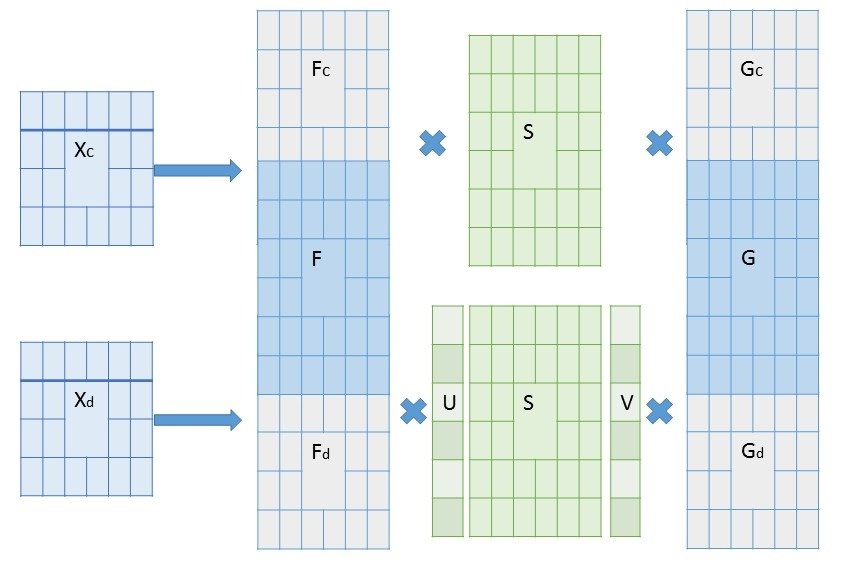
\includegraphics[width=400px]{fig/trimf.jpg} 
\caption{Graphical model of TRIMF}
\end{center}
\end{figure}}
 
  \par{Objective Function:$$min_{F,G,S,U,V} W_c\odot ||X_c - (F;F_c)S(G;G_c)'||_2 + W_d\odot ||X_d - (F;F_d)(USV)(G;G_d)'||_2 $$}

  \par{
    \begin{itemize}
    \item $W_c,W_d$ is the weight for $X_C, X_d$, every observed entry has weight $1 + log(frequency)$. while others have weight $W_{ij} = \sum_jI({R_{ij}})$.
    \item $F, G$ is the soft clustering result matrix for overlapped users(items), they are forced to have the same cluster distributions. Others are unique users(items).
    \item $U,V$ are two diagonal matrix, $U_{ii}$ scales every $S_{i*}$ to $U_{ii}S_{i*}$, it models the users' tranform from click to deal. While $V_{jj}$ scales every $S_{*j}$ to $S_{*j}V_{jj}$, it models the items' tranform from click to deal.
    \item When predicting, we use $(F;F_d)(USV)(G;G_d)$ to predict users who have deal data. And since we got two mapping matrix $U,V$, we apply $U,V$ back to click matrix to predict users who have click data, i.e we use $(F;F_c)(USV)(G;G_c)$ to predict.
    \end{itemize}
}



\begin{section}
  {Solution to TRIMF \& Algorithm}
\par{Follow the update rules in ~\cite{Zhuang:2011:EAW:1952191.1952195}, we use an alternately iterative algorithm to solve the objective function.}

Firstly, we declare some denotions:
\begin{itemize}
	\item $Ic,Icc,Icd,Id$ : $(Ic,Icc)*(F;F_c) = I*(F;F_c)$ and $(Icd,Id)*(F;F_d) = I*(F;F_d)$
	\item $sg$ : $S*G'*G*S'$
	\item $F_1, F_2$ : $[F;F_c]$, $[F;F_d]$
\end{itemize}
\par{In each round of iteration these matrixes are updated as :
$$F \leftarrow F .* \sqrt{\frac{Icc'*(W_c.*X_c)*G*S' + Icd'*(W_d.*X_d)*G*S'}{(Icc'*Icc*F + Icc'*Ic*F_c + Icd'*(Icd*F + Id*F_d))*sg)}}$$
$$F_c \leftarrow F_c .* \sqrt{\frac{Ic'*(W_c.*X_c)*G*S'}{Ic'*(Icc*F + Ic*F_c)*sg}}$$
$$F_d \leftarrow F_d .* \sqrt{\frac{Id'*(W_d.*X_d)*G*S'}{Id'*(Icd*F + Id*F_d)*sg }}$$
$$G \leftarrow G .* \sqrt{\frac{W_c.*X_c*F_1*S + (W_d.*X_d)'*F_2*S}{(G*(S'*F_1'*F_1*S + S'*F_2'*F_2*S)}}$$
$$U \leftarrow U .* \sqrt{\frac{F_2'*(W_d.*X_d)*G*V'*S'}{F_2'*F_2*U*S*V*G'*G*V'*S'}}$$
$$V \leftarrow V .* \sqrt{\frac{S'*F_2'*(W_d.*X_d)*G}{S'*F_2'*F_2*S*V*G'*G}} $$



}

\par{The user-item matrix is typically very sparse with $z \ll nm$ non-zero entries while $k$ is typically
also much smaller than n, m. By using sparse matrix multiplications and avoiding dense intermediate matrices, the updates can be very efficiently
and easily implemented. In particular, updating F, S, G each takes $O(k^2 (m + n) + kz)$ , and the algorithm usually reach convergence in less than 200 iterations.}

\begin{algorithm}[tb]
\caption{Algorithm for TRIMF.}
\begin{algorithmic}

\STATE {\bfseries Input:} $\X_{c}$, $\X_{d}$\\
$\X_{c} \in \mathbb{R}^{m_c\times n_c}$: the purchase data \\
$\X_{d} \in \mathbb{R}^{m_d\times n_d}$: the click data\\

\STATE {\bfseries Initialize:} Initialize $W_c, W_d$ : $(1+log(freq))$ for observed, $\sum_jI({R_{ij}})$ for unseen, $F,G,S,U,V$ : $random$, Set overlap numbers for users and items

\FOR{ $i$ = 1 to $T$}

\STATE update $F$

\STATE update $F_c$, $F_d$

\STATE  update $G$

\STATE  update $S$

\STATE  update $U, V$


\ENDFOR

\STATE {\bfseries Output:} $F,G,S,U,V$

\end{algorithmic}
\label{algorithm:TRIMF}
\end{algorithm}

\end{section}
\begin{section}{Experiment}
  \begin{subsection}{Datasets}

We select real data from an online shopping site: yixun.com \footnote{http://www.yixun.com}. We collect data for 6 months, the entire dataset consists 5,324,231 users and 643,123 items. The sparsity in click matrix is $0.06\%$, in purchase matrix is $0.0003\%$.

To check the effectiveness of TRIMF in short time and long time, we construct two smaller datasets.

\begin{itemize}

\item \textbf{Yixun short term data}: we select data from two weeks, 20130801-20130814. we sample a fraction of user by random, and remove those whose action frequency is too low(e.g only one click during this period). In the click matrix we have 16240 users and 1932 items. In the purchase matrix we have 2520 users and 1791 items. There are 2029 overlapped users and 1642 overlapped items. We train our model using data from first week and data from second week is used for testing.
\item \textbf{Yixun long term data}: we select 1012 active users through 6 months. In their long term actions, there are 6021 items which have been clicked and 1973 items boughted. We select the five latest purchasing items per user as test data, others as training data. There are 1503 overlapped items.

\end{itemize}
\end{subsection}

\begin{subsection}{Metrics}
We use $prec@5$ and $prec@10$ as our evaluation meatures. $prec@n$ is the precision of top-n results. Our main goal is to optimize for conversion rate(future purchase matrix), so the test is mainly done in the purchase matrix. However, since TRIMF can also optimize for source domain(click matrix), some test in click matrix is also conducted.

  
\end{subsection}

\begin{subsection}{Baseline methods}  

We divide baseline methods into non-transfer methods and transfer methods. All baseline methods are shown in Table \ref{baseline}.
\begin{table}

\begin{center}
  \begin{tabular}{|c|c|}
    \hline
    non-transfer methods & transfer methods\\
    \hline
    Most Popular, SVD, NMF, PMF, BPRMF, WRMF&CMF, TCF, TRIMF\\
\hline
  \end{tabular}
\end{center}
\caption{Baseline methods.}
\label{baseline}


\end{table}
\subsubsection{non-transfer methods}
\par{
  For all non-transfer methods, we use 3 combinations of matrix as our training matrix:{deal, click, deal+click}, and report their best performace. We choose parameters by cross validation.
  \begin{itemize}
    \item Most Popular: Most popular selects top-n items in global, and provide same recommendation results for each user.
    \item SVD ~\cite{paterek07}: Singular Value Decomposition(SVD) is a typical method used in recommender system, here PureSVD from Matlab is used.
      \begin{itemize}
      \item rank = \{5,10,20,30,40,50\}
      \end{itemize}
    \item NMF ~\cite{/computer/yehuda09matrix}: Non-negative Matrix Factorization(NMF) is also a typical method used in recommender system, here NMF from Matlab is used.
      \begin{itemize}
      \item rank = \{10,20,40,60,100\}
      \end{itemize}
    \item PMF ~\cite{/nips/SalMnih08}:Probabilistic Matrix Factorization(PMF) is a recently proposed method for missing value prediction. Previous work showed that this method worked well on the large, sparse and imbalanced data set.
      \begin{itemize}
      \item rank = \{10,20,30,40,50\}
      \end{itemize}
    \item BPRMF ~\cite{Rendle:2009:BBP:1795114.1795167}: BPR is a generic optimization criterion for personalized ranking that is the maximum posterior estimator derived from a Bayesian analysis of the problem. Unlike traditional methods whose object function is point-wise, BPR is a pair-wise object function. BPRMF implements BPR using matrix factorization.
      \begin{itemize}
      \item We initialized BPR with most popular results.
      \item We set $iteration = \#n * 100$, ($\#n$ in the number of observations)
      \end{itemize}
    \item WRMF ~\cite{4781145}: One-class collaborative filtering(WRMF) is a weighted low rank approximation method optimized for implicit dataset. 
      \begin{itemize}
      \item rank = \{5,10,15,20,25\}
    \end{itemize}
\end{itemize}
\subsubsection{transfer methods}
\begin{itemize}
    \item CMF ~\cite{/kdd/SinghG08}:Collective Matrix Factorization is proposed for jointly factorizing two matrices. Being adopted as a transfer
learning technique in several recent works, CMF has been proven to be an effective cross-domain recommendation approach. For each training and testing pairs, we make two matrix the same dimension(in order to share a latent factor) by padding rows \& columns.
      \begin{itemize}
      \item Shared latent space dimension = \{5,10,15,20,25\}
      \end{itemize}
    \item TCF ~\cite{/ijcai/PanLXY11}: TCF is a transfer learning method to predict missing ratings via heterogeneous feedbacks. It's originally designed for rating prediction, so we set the deal matrix with random sampled zeros as the rating matrix, click matrix as the implicit feed back matrix. Zero rows and colomns are also padded to make the two matrix in same dimension.
\item TRIMF: our method.
  \begin{itemize}
  \item We set latent factor = 30, iteration = 200.
  \end{itemize}
    \end{itemize}
  
}
\end{subsection}
\end{section}
\subsection{Results}
  \begin{subsubsection}{Yixun short term data}
\par{Since the user overlap of deal and click matrix are small, so we perform two test, one on deal matrix $X_d$ and one on click matrix $X_c$.}
\par{Results are showed in Table \ref{shortdeal} and Table \ref{shortclick}.}
\begin{table}


\begin{center}
  \begin{tabular}{|c|c|c|}
    \hline
    Method&Prec@5&Prec@10\\
    \hline
    Most Popular&0.0323&0.0289\\
    \hline
    SVD&0.0438&0.0367\\
    \hline
    NMF&0.0403&0.0324\\
    \hline
    PMF&0.0435&0.0372\\
    \hline
    BPRMF&0.0444&0.0364\\
    \hline
    WRMF&0.049&0.0403\\
    \hline
    CMF&0.0436&0.0350\\
    \hline
    TCF&0.0453&0.0369\\
    \hline
    TRIMF&\textbf{\color{red}0.0525}&\textbf{\color{red}0.0410}\\
    \hline
  \end{tabular}
\end{center}
\caption{Performance of TRIMF and other baseline methods on short-term users who have deal data.}
\label{shortdeal}

\end{table}

\begin{table}

  \centering


  \begin{tabular}{|c|c|c|}
    \hline
    Method&Prec@5&Prec@10\\
    \hline
    Most Popular&0.0090&0.0085\\
    \hline
    SVD&0.0123&0.00113\\
    \hline
    NMF&0.0091&0.0089\\
    \hline
    PMF&0.0121&0.0112\\
    \hline
    BPRMF&0.0142&0.0130\\
    \hline
    WRMF&0.0174&0.0144\\
    \hline
    CMF&0.0176&0.0139\\
    \hline
    TCF&0.0158&0.0127\\
    \hline
    TRIMF&\textbf{\color{red}0.0189}&\textbf{\color{red}0.0153}\\
    \hline
    TRIMF(without remap)&0.0175&0.0146\\
    \hline
  \end{tabular}
\caption{Performance of TRIMF and other baseline methods on short-term users who have deal data.}
  \label{shortclick}
  
\end{table}
\end{subsubsection}


\begin{subsubsection}
  {Yixun long term data}
\par{Since the user are manually selected, we only test $X_d$. The result is showed in Table \ref{longterm}.}

\begin{table}
  \centering
  \begin{tabular}{|c|c|c|}
    \hline
    Method&Prec@5&Prec@10\\
    \hline
    Most Popular&0.00508&0.00405\\
    \hline
    SVD&0.00453&0.00413\\
    \hline
    NMF&0.00401&0.00389\\
    \hline
    PMF&0.00421&0.00312\\
    \hline
    BPRMF&0.00542&0.00430\\
    \hline
    WRMF&0.00485&0.00345\\
    \hline
    CMF&0.00512&0.00432\\
    \hline
    TCF&0.00534&0.00502\\
    \hline
    TRIMF&\textbf{\color{red}0.00720}&\textbf{\color{red}0.00606}\\
    \hline
  \end{tabular}
  \caption{Performance of TRIMF and other baseline methods on long-term users.}
\label{longterm}
\end{table}
\end{subsubsection}



\begin{section}{Performance comparison \& analysis}
First, we observed that TRIMF out-perform all other baseline non-transfer methods in three tests. In short-term deal test, we can see traditional CF method which aims at rating prediction (e.g SVD, NMF) can't achieve compatible performance than others. Because these methods is designed for matrix with multiple values, not for our binary matrix. while CF method designed for binary matrix(BPRMF, WRMF) can acheive significantly greater result. In long-term test the difference is not so significant, because the data here is less sparse than short-term data, every method has enough data to train a good model.

Second, TRIMF also out-perform other transfer methods. Since CMF, TCF are also designed for rating prediction problems. The information in our training set is limited, so both methods can't transfer enough knowledge from their framework. TRIMF is designed for one-class transfer learning, TRIMF combines one-class and transfer methods, so it inherits advantages from both side.

  \subsubsection{The effects of $UV$}
In our assumption, $UV$ are two mapping matrix that describe the difference in user-cluster and item-category. To see whether $UV$ really reflects the phenomenon, we manually check entries in $UV$ with high and low values.

  We found that high value in $V$ reflects item clusters that people tends to buy after clicking, e.g toothbrush, snacks. While low value of $V$ more reflects that items are popular but people may not buy it immediately, e.g cell phones, laptops. High value in $U$ reflects user-cluster who tends to buy after clicking, while users belong to low value user-clusters are all window-shopping fans.

  In Table \ref{shortclick}, we can see if we want to predict future purchasing items on users who have click data, we can map $UV$ back. Thus the learned cluster-pattern $S$ is transformed from click pattern to purchase pattern.

  \subsubsection{The effects of sharing}
    To see that sharing $F,G$ really works, we select another 6000 users to test, we tried 'not share','share' and 'random share', the $prec@n$ here are not comparable with the first experiment(Table \ref{shortdeal}). Results show that we must share latent factor carefully, random share may do harm to performance. But sharing latent factor for overlapped users/items can achieve a significantly greater result.

    \par{
\begin{table}
\begin{center}
  \begin{tabular}{|c|c|c|}
    \hline
    Method&Prec@5&Prec@10\\
    \hline
    shareFG&\textbf{\color{red}0.0436}&\textbf{\color{red}0.0350}\\
    \hline
    not share&0.0335&0.0306\\
    \hline
    random share&0.0344&0.0299\\
    \hline
  \end{tabular}
\end{center}
\caption{The effect of sharing}
\label{sharing}
\end{table}
}
\end{section}


\chapter{Clustering-based Matrix Factorization for Online Shopping Prediction}
\label{chp:cbmf}
\section{Limitation of TRIMF}
In Chapter \ref{chp:trimf}, we introduced TRIMF, which is a matrix tri-factorization method for cross-domain recommendation. However, it has some limitations which restrict its scalability and extensibility. First, when data are coming from multiple sources (e.g. click, pageview and add cart), TRIMF treats every source equally and puts each of them into a matrix which is very sparse. When solving the object function, increasing the matrixes will increase the time and space complexity. If we try to update $S$, every matrix is included so it will be quite time-consuming. What is more, in reality we cannot ignore users with fewer actions. Thus, the matrix will be much more sparse than the ones in our experiment, so we cannot guarantee achieving equal performance.

To solve these problems, we have developed a framework based on a clustering and scoring scheme (CBMF, Figure \ref{fig:cbmf}). CBMF first clusters users according to their behaviors and demographic features, then automatically converts different types of actions into one matrix, called action matrix. Finally a matrix factorization method is applied to the action matrix. For users with adequate actions, a personalized recommendation is provided. Otherwise we provide a recommendation based on their clusters.

We conduct two experiments: 
\begin{itemize}
\item offline experiment: we select datasets used in TRIMF, and compare the run-time and precision of the two methods.
\item online experiment: we do A/B test with CBMF in an online shopping site.
\end{itemize}
Results show that in offline datasets, CBMF runs much faster then TRIMF while achieving equal performance. In online test, CBMF outperforms other methods in conversion rate.


\begin{figure}

%\begin{Large}

\begin{center}
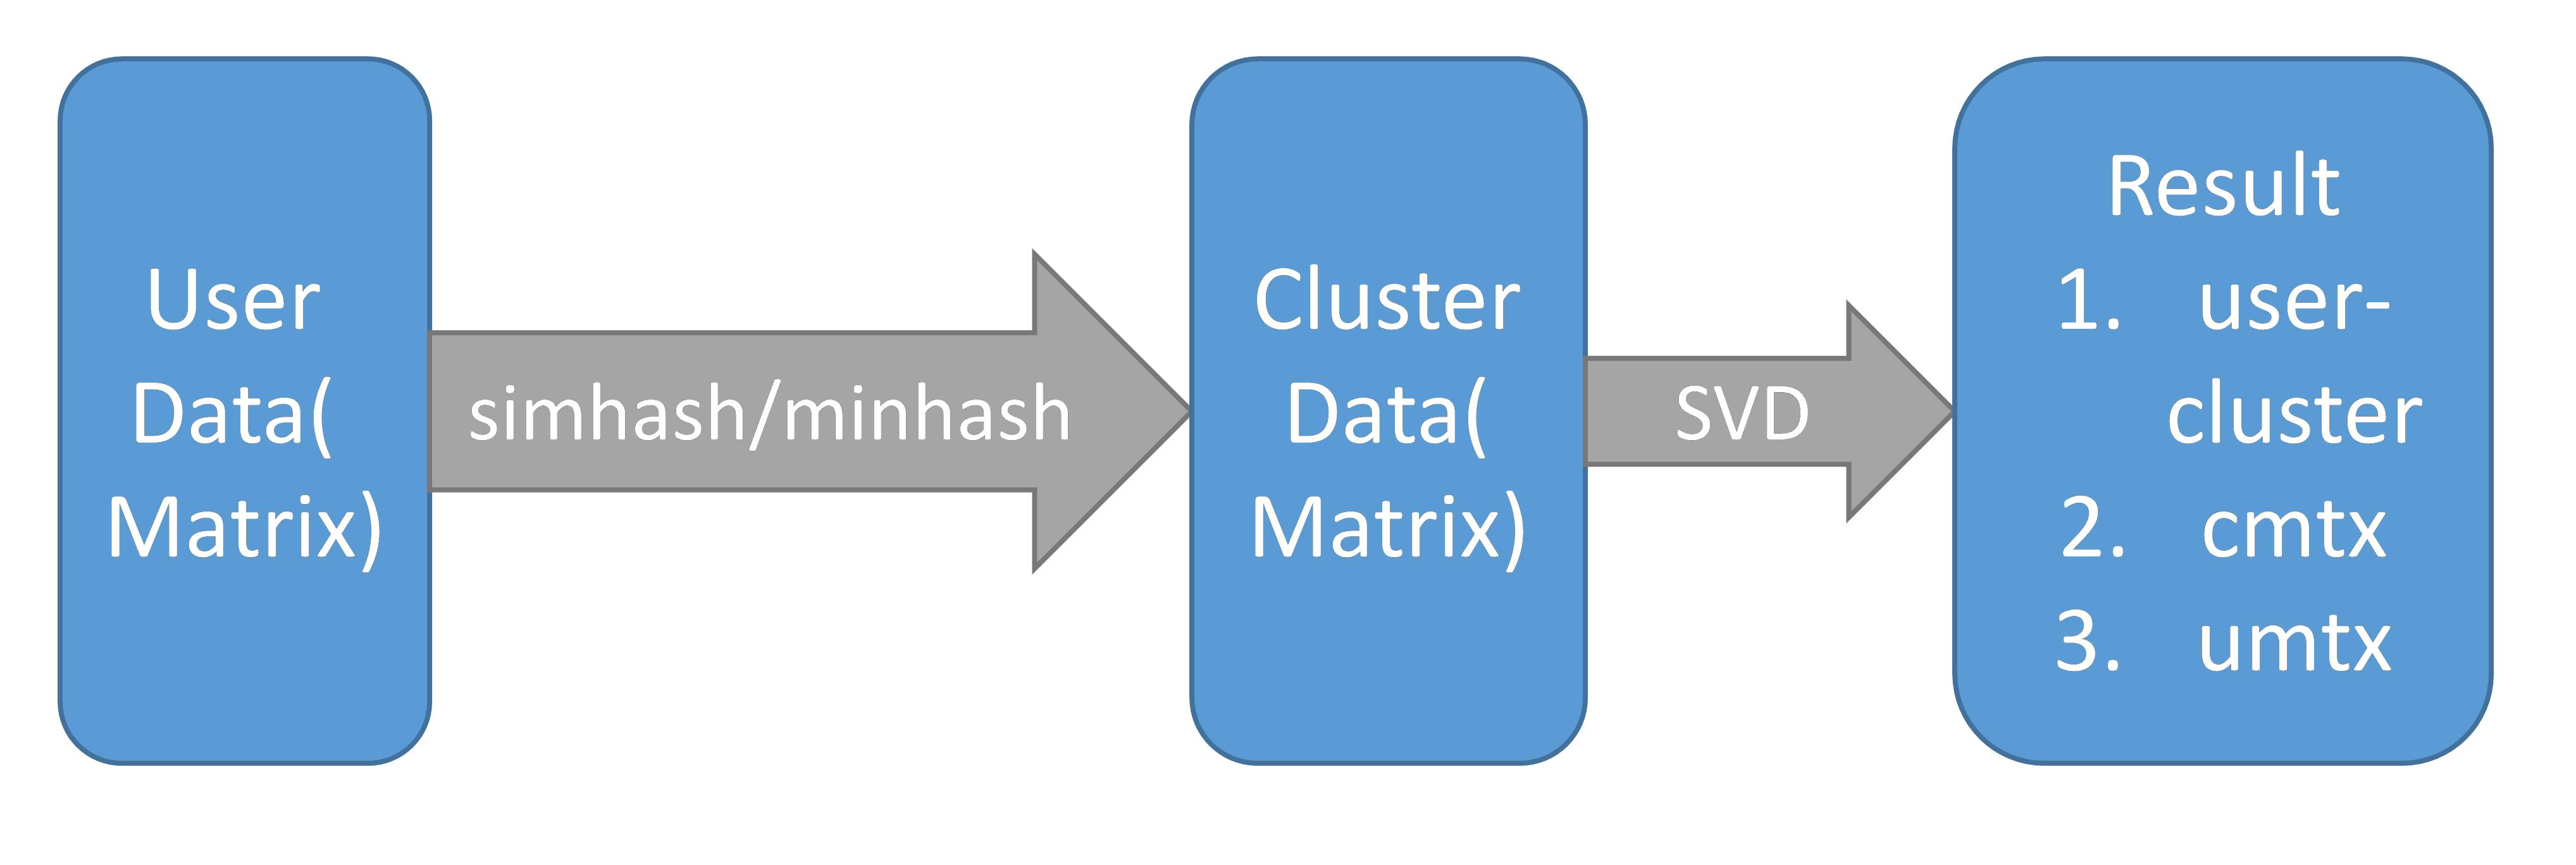
\includegraphics[width=400px]{fig/d} 
\caption{Framework of CBMF.}
\label{fig:cbmf}
\end{center}
\end{figure}





\section{Clustering method in CBMF}

Usually users’ actions are unique and sparse and it would be time-consuming if we want to cluster users by using raw data. In Tencent, we have 800,000,000 users in total, and their feature vectors dimensions can be as large as 1,000,000. Therefore, if we want to speed up the phase, we must first convert large sparse user vector into a low dimensionally dense vector.

\subsection{Simhash}

Simhash is a kind of locality sensitive hashing(LSH). LSH is a hashing method where if we got two points $A,B$ which are close in their original space, after hashing we would get $A',B'$, with $A',B'$ still close in the new space. Thus we keep the relationship of distance among the two spaces. 

The input of Simhash per user is $(feature_1, weight_1),..(feature_n,weight_n)$. The procedure of Simhash is in Algorithm \ref{algorithm:simhash}.

\begin{algorithm}[tb]
\caption{Simhash Algorithm for one instance.}
\begin{algorithmic}

\STATE {\bfseries Input:} $\X_U$, $h$\\
$\X_{U}$ : $(feature_1, weight_1),..(feature_n,weight_n)$ \\
$h$: a smooth hash function with $k$ bits after hashing\\

\STATE {\bfseries Initialize:} $r$(result vector) : $[0,0,0..0] \in \{0,1\}^k$

\FOR{ $i$ = 1 to $n$}

\STATE calculate $h(feature_i)$

\STATE $r = r + weight_i * h(feature_i)$

\ENDFOR

\FOR{ $i$ = 1 to $k$}
\IF {$r_i > 0$}
\STATE {$r_i = 1$}
\ELSE 
\STATE {$r_i = 0$}
\ENDIF
\ENDFOR

\STATE {\bfseries Output:} $r$

\end{algorithmic}
\label{algorithm:simhash}
\end{algorithm}

Assume that Simhash converts a vector $x$ into a 32-dimension binary vector $x'$. Actually $i_{th}$ bit of $x'$ is the sign of the inner product of $x$ and $H_i = [h^1_i, h^2_i,...h^n_i]$, $H_i$ can be regarded as a hyperplane in original space. If two vectors $x, y$ are in the same direction of $H_i$, then $x', y'$ is equal on $i_{th}$ bit. Thus we can use hamming distance in the new space to represent their similarity in original space.

\subsection{Minhash}

The similarity between two users $u_i , u_j$ is defined as the overlap between their item sets. $S(u_i, u_j) = \frac{C_{u_i} \cup C_{u_j}}{C_{u_i} \cap C_{u_j}}$, also known as the Jaccard coefficient. Regardless, calculating all similarities in real-time is nearly impossible. However, we can achieve a provably sublinear time near-neighbor search technique by applying Minhash.

MinHash is a probabilistic clustering method that assigns a pair of users to the same cluster with a probability proportional to the overlap between the set of items that these users have voted for (clicked-on). In CBMF, Minhash is applied after Simhash and every user vector consists of 32 bits. 

The basic idea in the Minhash scheme is to randomly permute the set of items (S) and for each user $u_i$ compute its hash value $h(u_i)$ as the index of the first item under the permutation that belongs to the user’s item set $C_{u_i}$. It is also easy to prove that the probability of two users having the same hash function is exactly equal to their similarity or Jaccard coefficient.Similar to \cite{Indyk:1998:ANN:276698.276876}, we can always concatenate $p$ hash-keys for
users, where $p \ge 1$, so the probability that any two users $u_i , u_j$ will agree the concatenated hash-key is equal to $S(u_i , u_j )^p$. In that case, $p$ can be a parameter to control the number of clusters. If $p$ is large, then the clusters will be more refined thus the number of clusters will increase.

\subsection{Simhash \& Minhash using MapReduce}

MapReduce is a model of computation over large clusters of machines that can handle processing of large amounts of data in relatively short periods of time and scales well with the number of machines. Our method Simhash and Minhash can easily be implemented using hadoop.

\subsubsection{Map phase}
In the map phase, we read the input records independently, in parallel, on different machines and map each input to a set of key-
value pairs. In our case, hadoop streaming is applied and each input instance is a user's vector(in sparse representation).

We first iterate the user's vector $u_i$, using Simhash to convert the vector to a 32-bit binary vector, the hashing function used in Simhash is FNV-32. Then Minhash is applied $p$ times per user. We concatenate the $p$ Minhash values $Mnhs_i$ to obtain the cluster id of the user. Finally, the output is ( $Mnhs_i$, $u_i$), key is $Mnhs_i$, value is $u_i$. For users with enough actions, we output another pair ( $user-id$, $u_i$). 

\subsubsection{Reduce phase}

In the reduce phase, our input takes two forms: ($Mnhs_i$, $u_i$) represents cluster-id and user vector. ($user-id$, $u_i$) represents an experienced user and his vector.
\begin{itemize}
\item In the cluster case: for each cluster-id we obtain the list of user-ids that belong to this cluster and prune away clusters with members less than 10. For each cluster-id, a joint vector is needed to represent all users in it. Thus we simply add scores from users to the joint vector. We, then do a normalization sothe range of the vector is between 0 and 1. The output has two parts: 
\begin{itemize}
\item users and the cluster they belong to (userid, clusterid). 
\item cluster-ids and their vectors (cluster-id, cluster-vector).
\end{itemize}
\item In the user case: we simply output the normalized vector.

\end{itemize}

After the reduce phase, we have three tables(matrices). 1, user and the respective cluster-id; 2, cluster-id and its vector; 3, user and respective vector.

\section{Feature construction in CBMF}

After clustering, we have many clusters and their corresponding actions, including click, purchase and pageview on different (overlapping) items.

The naive way to handle those actions is to create a matrix $X_i$ for each action $i$. In matrix $X_i$, a row represents a cluster while a column represents an item, $X_{mn}$ represents the frequency of action that users in cluster $m$ used on item $n$. However, simply creating such a matrix may lead to data sparsity problems. This is especially true in the matrix standing for purchasing actions, even though similar users are alredy clustered together.The data is still very sparse($0.01\%$) which may constrain our model from providing a reasonable recommendation.

In CBMF, a scoring scheme is applied for each kind of action to put every action into a single matrix with a proper score. For a specific item, a user may have four kinds of actions (click, purchase, pageview and uninterested). The idea behind the construction is that for a specific goal (e.g predict future purchase), the score that should be given to an action depends on how much impact the action can have.

For example, if we want to improve conversion rate, let $U_n$ denote the users who bought item $n$, while $U$ denotes the entire user set. The average conversion rate for a given item $n$ can be approximated by $Cvr(n_{all}) \approx \frac{|U_n|}{|U|}$. 
For a given action(e.g. click), let $U_n^{click}$ denote the users who clicked item $n$. Then the conversion rate for users who had clicked these items can then be approximated by $Cvr(n_{click}) \approx \frac{|U_n \cap U_n^{click}|}{|U_n^{click}|}$we compare the conversion rate of users with this action with the average, and their log ratio $log(\frac{Cvr(n_{click})}{Cvr(n_{all})})$ is our initial score.

For each action with an item we calculate a score, in CBMF we use weighted scores and add them together. That is, for cluster $m$ and item $n$, if we have four scores:$s_1, s_2, s_3, s_4$ and their corresponding weights:$w_1, w_2, w_3, w_4$. $w_i$ is the percentage of users who have this action compared to all users. The result, $X_{mn} = \frac{\sum_{i=1}^4 w_i*s_i}{\sum_{i=1}^4 w_i}$. 

\section{Matrix factorization in CBMF}

Once the matrices are generated, we use Singular Value Decomposition(SVD) from mahout \footnote{https://mahout.apache.org/users/dim-reduction/dimensional-reduction.html}. The number of eigenvalues is set to 20 according to the online test.

After SVD, we can provide recommendations to every user; for experienced users direct results are provided, otherwise we find the user's cluster-id and provide results for this cluster as our recommendation. We output our results to an online key-value dataset called TDE. Once a user comes, we search his id in TDE, and the return value is our recommendation.



%
\chapter{Experiments}
\label{chp:exp}

\hspace{0.1in}
\section{Data Sets and Experimental Settings} \label{sec:DataSets}
We evaluate the proposed method on four data sources:
Netflix\footnote{http://www.netflix.com},
Douban,
IMDB\footnote{http://www.imdb.com},
and Wikipedia\footnote{http://en.wikipedia.org} user editing records.
The Netflix rating data contains more than $100$ million ratings with values in $\{1, 2, 3, 4, 5\}$, which are given by more than $4.8\times 10^5$ users
on around $1.8\times 10^4$ movies.
Douban contains movie, book and music recommendations, with rating values also in $\{1, 2, 3, 4, 5\}$.
IMDB hyperlink graph is employed as a measure of similarity between movies.
In the graph, each movie builds links to its $10$ most similar movies.
%The value $1$ is used to denote the top $10$ most similar movies for each movie in the movie-to-movie matrix.
The Wikipedia user editing records provide a $\{0, 1\}$ indicator of whether a user concerns or not about a certain movie.

The data sets used in the experiments are described as follows. For Netflix, to retain the original features of the users while keeping the size of the data set suitable for the experiments, we sampled a subset of $10,000$ users.
In Douban data sets, we obtained $1.2 \times 10^6$ ratings on $7.5 \times 10^3$ music, $ 5.8 \times 10^5 $ ratings on $3.5 \times 10^3 $ books, and $1.4 \times 10^6 $ ratings on $8 \times 10^3$ movies, given by $1.1 \times 10^4 $ users.
For both the IMDB data set and the Wikipedia data set, we filtered them by matching the movie titles in both the Netflix and the Douban Movie data sets. After pre-processing, the IMDB hyperlink data set contains $\sim 5 \times 10^3$ movies. The Wikipedia user editing records data set has $1.1 \times 10^6$ editing logs by $8.5 \times 10^3$ users on the same $\sim 5 \times 10^3$ movies as IMDB data set.
To present our experiments, we use the shorthand notations listed in Table \ref{tbl:notationDataset} to denote the data sets.


%%%%%%%%%%%%%%%%%%%%%%%%%%%-=Table1=-%%%%%%%%%%%%%%%%%%%%%%%%

\begin{table}[!tbp]
\caption{Datasets in our experiments.}
\label{tbl:notationDataset}
\begin{Large}
\begin{center}
\begin{tabular}{ c | c | c |c}
\hline\hline
Notation & Data Set & Data Type & Instances No. \\
\hline \hline
D1 & Douban Music & Rating [1,5]& $1.2 \times 10^6$\\
D2 & Douban Book & Rating [1,5]& $5.8 \times 10^5$ \\
D3 & Douban Movie & Rating [1,5]& $1.4 \times 10^6$ \\
D4 & Netflix & Rating [1,5]& $1.8 \times 10^4$\\
D5 & Wikipedia & Editing Log & $1.1 \times 10^6$\\
D6 & IMDB & Hyperlink & $5.0 \times 10^3$\\
\hline\hline
\end{tabular}
\end{center}
\end{Large}
\end{table}
%%%%%%%%%%%%%%%%%%%%%%%%%%%%%%%%%%%%%%%%%%%%%%%%%%%%%%%%%%

We evaluate the proposed algorithm on five cross-domain recommendation tasks, as follows:
\begin{itemize}[noitemsep,topsep=0pt,parsep=0pt,partopsep=0pt]
\item The first task is to simulate the cross-domain collaborative filtering, using the Netflix data set. The sampled data is partitioned into two parts with disjoint sets of movies but identical set of users. One part consists of ratings given by $8,000$ movies with $1.6\%$ density, which serves as the source domain. The remaining $7,000$ movies are used as the target domain with different levels of sparsity density.
\item The second task is a real-world cross-domain recommendation, where the source domain is Douban Book and the target domain is Douban Movie. In this setting, the source and the target domains share the same user set but have different item sets.
\item The third task is on Netflix and Douban data. We extract the ratings on the $6,000$ shared movies from Netflix and Douban Movie. Then we get $4.9 \times 10^5$ ratings from Douban given by $1.2 \times 10^4$ users with density $0.7\%$, and $10^6$ ratings from Netflix given by $10^4$ users with density $1.7\%$. The goal is to transfer knowledge from Netflix to Douban Movie. In this task, item set is identical across domains but user sets are totally different.
\item The fourth task is to evaluate the effectiveness of the proposed algorithm under the context of multiple source domains. It uses both Douban Music and Douban Book as the source domains and transfer knowledge to Douban Movie domain.
\item The fifth task varies the type of source domains. It utilizes the Wikipedia user editing records and IMDB hyperlink graph, together with Douban Movie as the source domains to perform rating predictions on the Netflix movie data set.
\end{itemize}

For evaluation, because we adopt the error rate style objective function in our optimization, we calculate the Root Mean Square Error (RMSE) on the heldout $\sim 30\%$ of the target data:
\begin{eqnarray}
    RMSE &=& \sqrt{ \sum_{ (u, i, x_{ui}) \in T_E } (x_{ui} - \hat{x}_{ui})^2 / |T_E|} \nonumber
\end{eqnarray}
where $x_{ui}$ and $\hat{x}_{ui}$ are the true and predicted ratings, respectively, and $|T_E|$ is the number of test ratings.



%%%%%%%%%%%%%%%%%%%%%%%%%%%-=Table2=-%%%%%%%%%%%%%%%%%%%%%%%%
\begin{table*}[!tbp]
\caption{Prediction performance of STLCF and the baselines.}
\label{tbl:TLCF}
\begin{footnotesize}
\begin{center}
\begin{tabular}{ c || c || c || c c || c c || c  c } \hline\hline

% ************************************************************************************************
 \multirow{2}{*}{Datasets}
& \multirow{1}{*}{Source}
& \multirow{1}{*}{Target}
& \multicolumn{2}{c ||}{Non-TL}
& \multicolumn{2}{c ||}{Non-Selective TL}
& \multicolumn{2}{c }{\bf Selective TL}\\
\cline{4-9}
% \hline \hline
% \hline \hline
&sparseness
&sparseness
& \multicolumn{1}{c }{GPLSA}
& \multicolumn{1}{c||}{PMF}
& \multicolumn{1}{c }{TGPLSA}
& \multicolumn{1}{c||}{CMF}
& \multicolumn{1}{c }{STLCF(E)}
& \multicolumn{1}{c}{STLCF(EV)}\\
\hline \hline
D4(Simulated) & \multirow{3}{*}{1.6\%} & 0.1\% & 1.0012 & 0.9993 & 0.9652 & 0.9688 & 0.9596 & \textbf{0.9533} \\
\cline{3-9}
to      &                        & 0.2\% & 0.9839 & 0.9814 & 0.9528 & 0.9532 & 0.9468 & \textbf{0.9347} \\
\cline{3-9}
D4(Simulated) &                        & 0.3\% & 0.9769 & 0.9728 & 0.9475 & 0.9464 & 0.9306 & \textbf{0.9213} \\
\hline \hline
& \multirow{3}{*}{1.5\%} & 0.1\% & 0.8939 & 0.8856 & 0.8098 & 0.8329 & 0.7711 & \textbf{0.7568} \\
\cline{3-9}
D2 to D3&                        & 0.2\% & 0.8370 & 0.8323 & 0.7462 & 0.7853 & 0.7353 & \textbf{0.7150} \\
\cline{3-9}
&                        & 0.3\% & 0.7314 & 0.7267 & 0.7004 & 0.7179 & 0.6978 & \textbf{0.6859} \\
\hline \hline
& \multirow{3}{*}{1.7\%} & 0.1\% & 0.8939 & 0.8856 & 0.8145 & 0.8297 & 0.7623 & \textbf{0.7549} \\
\cline{3-9}
D4 to D3 &                        & 0.2\% & 0.8370 & 0.8323 & 0.7519 & 0.7588 & 0.7307 & \textbf{0.7193} \\
\cline{3-9}
&                        & 0.3\% & 0.7314 & 0.7267 & 0.7127 & 0.7259 & 0.6982 & \textbf{0.6870} \\
\hline \hline

\end{tabular}
\end{center}
\end{footnotesize}
\end{table*}
%%%%%%%%%%%%%%%%%%%%%%%%%%%%%%%%%%%%%%%%%%%%%%%%%%%%%%%%%%

\hspace{0.1in}
\section{STLCF and Baselines Methods}
We implement two variations of our STLCF method.
STLCF(E) is an STLCF method that only take training error into consideration when performing selective transfer learning.
STLCF(EV) not only considers training error, but also utilizes the empirical error variance.

To demonstrate the significance of our STLCF, we selected the following baselines:
\begin{itemize}
\item {\bf PMF}~\cite{/nips/SalakhutdinovM07} is a recently proposed method for missing value prediction. Previous work showed that this method worked well on the large, sparse and imbalanced data set.
\item {\bf GPLSA}~\cite{DBLP:conf/sigir/Hofmann03} is a classical non-transfer recommendation algorithm.
\item {\bf CMF}~\cite{/kdd/SinghG08} is proposed for jointly factorizing two matrices. Being adopted as a transfer learning technique in several recent works, CMF has been proven to be an effective cross-domain recommendation approach.
\item {\bf TGPLSA} is an uniformly weighted transfer learning model, which utilize all source data to help build the target domain model. It is used as one of the baselines because we adopt it as the base model of our boosting-based selective transfer learning framework.
\end{itemize}
Parameters for these baseline models are fine-tuned via cross validation.

\hspace{0.1in}
\section{Experimental Results}
\subsection{Performance Comparisons}
We test the performance of our STLCF methods against the baselines.
The results of the collaborative filtering tasks under three different target domain sparseness are shown in Table \ref{tbl:TLCF}.

First, we observe that the non-transfer methods, i.e. GPLSA and PMF, fail to give accurate predictions, especially when the target domain is severely sparse.
With the help of source domains, the (non-selective) transfer learning methods with equally weights on the source domains, like TGPLSA and CMF, can increase the accuracy of the rating predictions. And our selective transfer learning methods (i.e., STLCF(E) and STLCF(EV)) can do even better.
The fact that our STLCF outperforms others is expected because by performing the {\em selective} knowledge transfer, we use the truly helpful source domain(s), which is designed to handle the sparseness issue in CF problems.

Second, comparing the two non-selective TLCF methods with the other two selective TLCF methods, we observe that on the last two real world tasks (D2 to D3 and D4 to D3) when the target domain is extremely sparse (say 0.1\%), the improvement of accuracy achieved by our STLCF methods against the non-selective transfer learning methods is more significant than it does on the simulation data set based on Netflix (D4 to D4).
Notice that the inconsistency of the target domain and the source domains on the simulation data sets is much smaller than that on the real-world cases. The experiment results show that our STLCF algorithm is effective in handling the inconsistency between the sparse target domain and the source domains.

Third, we notice that some factors, like empirical error variance, may affect the prediction. In Table \ref{tbl:TLCF}, we compare our two STLCF methods, i.e., STLCF(E) and STLCF(EV) when the target domain sparsity is $0.1\%$. We can find that on the task ``D2 to D3", i.e., Douban Book to Movie, STLCF(EV) is much better than STLCF(E). But on the task ``D4(Simulated) to D4(Simulated)", the improvement of STLCF(EV) is not so significant against STLCF(E). These observations may be due to the domain consistency.
For the tasks ``D4(Simulated) to D4(Simulated)", both the source and target entities are movie ratings from Netflix data set, while the task ``D2 to D3" tries to transfer the knowledge from a book recommendation system to the movie recommendation system, which may contain some domain specific items.
When the target domain is very sparse, i.e. the user's ratings on the items are rare, there are chances to get high prediction accuracy occasionally on the observed data with a bad model on the source domains that are inconsistent with target domain. In this case, it is important to consider the variance of empirical error as well. Comparing to STLCF(E), STLCF(EV), which punishes the large variance, can better handle the domain inconsistency in transfer learning, especially when the target domain is sparse.

\hspace{0.05in}
\subsection{Results on Long-Tail Users} \label{sec:long-tail}
%%%%%%%%%%%%%%%%%%%%%%%%%%%-=Table3=-%%%%%%%%%%%%%%%%%%%%%%%%%%%%%%%
\begin{table} [t]
\begin{LARGE}
\caption{Prediction performance of STLCF for Long-Tail Users on the D2 to D3 task.}
\label{tbl:tail}
\begin{center}
\begin{tabular}{l||c|| cc||cc}
\hline\hline
Ratings & \multirow{1}{*}{\multirow{2}{*}{Non-TL}} & \multicolumn{2}{c ||}{\multirow{2}{*}{Non-Selective TL}} & \multicolumn{2}{c}{\bf Selective TL}\\
%\cline{3-6}
per & & & & \multicolumn{2}{c} {\bf i.e. STLCF}\\
\cline{2-6}
user & GPLSA & TGPLSA & CMF & (E) & (EV)\\
\hline\hline
1-5   & 1.1942 & 0.9294 & 0.9312 & 0.8307 & \textbf{0.8216}\\\hline
6-10  & 0.9300 & 0.7859 & 0.7929 & 0.7454 & \textbf{0.7428}\\\hline
11-15 & 0.8296 & 0.7331 & 0.7390 & \textbf{0.7143} & 0.7150\\\hline
16-20 & 0.7841 & 0.7079 & 0.7113 & \textbf{0.7042} & 0.7050\\\hline
21-25 & 0.7618 & 0.6941 & 0.6947 & 0.6942 & \textbf{0.6910}\\\hline
26-30 & 0.7494 & 0.6918 & 0.6884 & 0.6917 & \textbf{0.6852}\\\hline
31-35 & 0.7370 & 0.6909 & 0.6911 & 0.6915 & \textbf{0.6818}\\\hline
36-40 & 0.7281 & 0.6896 & 0.6856 & 0.6907 & \textbf{0.6776}\\\hline
41-45 & 0.7219 & 0.6878 & 0.6821 & 0.6890 & \textbf{0.6740}\\\hline
46-50 & 0.7187 & 0.6881 & 0.6878 & 0.6800 & \textbf{0.6734}\\
\hline
\hline
\end{tabular}
\end{center}
\end{LARGE}
\end{table}
%%%%%%%%%%%%%%%%%%%%%%%%%%%%%%%%%%%%%%%%%%%%%%%%%%%%%%%%%%
To better understand the impact of STLCF with the help of the source domain, we conduct a fine-grained analysis on the performance improvement on Douban data sets, with Douban Book as source domain and Douban Movie as target domain.
The results on different user groups in the target domain are shown in Table \ref{tbl:tail}. In the table, method STLCF(E) does not punish the large variance of empirical error, while STLCF(EV) does.
%The overall data sparsity for the target domain is 0.4\%.
First, we observe that the STLCF models, i.e., STLCF(E) and STLCF(EV) can achieve better results on those long-tail users who have very few ratings in historical logs.
Such fact implies that our STLCF methods could handle the long-tail users that really need a fine-grained analysis when performing knowledge transfer from source domains.
Current CF models without any fine-grained analysis on the specific users usually fail to capture the preferences of the long-tail users, while our STLCF methods work well because they can selectively augment the weight of the corresponding source domain instances with respect to those long-tail cases at both instance level and domain level.
Second, STLCF(EV) works better than STLCF(E) on those non-long-tail users, i.e., with more than 25 ratings per user in the historical log. This is expected because users with more ratings can benefit more from the error variance analysis to avoid negative knowledge transfer.
%%%%%%%%%%%%%%%%%%%%%%%%%%%-=Table4=-%%%%%%%%%%%%%%%%%%%%%%%%%%%%%%%
\begin{table*}[t]
\caption{Prediction performance of STLCF with multiple source domains containing much irrelevant information.}
\label{tbl:mdomainshyb}
\begin{center}
\begin{tabular}{ c | c || c || c | c | c | c | c }
\hline\hline
\multicolumn{2}{c ||} {Source Domain: }  & None  & D3 & D3 \& D5 & D3 \& D6 & D5 \& D6 & D3 \& D5 \& D6\\
\hline\hline
 \multirow{1}{*}{Target} & 0.1\% & 0.9983 & $0.9789$& $0.9747$& $0.9712$& $0.9923$&$\textbf{0.9663}$\\
\cline{2-8}
 \multirow{1}{*}{(D4)} & 0.2\% & 0.9812 & $0.9625$& $0.9583$&$0.9572$ & $0.9695$ & $\textbf{0.9505}$\\
\cline{2-8}
 \multirow{1}{*}{sparseness} & 0.3\%& 0.9703 & $0.9511$& $0.9409$& $0.9464$& $0.9599$ &$\textbf{0.9383}$\\
\hline\hline
\end{tabular}
\end{center}
\end{table*}
%%%%%%%%%%%%%%%%%%%%%%%%%%%%%%%%%%%%%%%%%%%%%%%%%%%%%%%%%%


%%%%%%%%%%%%%%%%%%%%%%%%%%%-=Table5=-%%%%%%%%%%%%%%%%%%%%%%%%%%%%%%%
\begin{table}[!tbp]
\caption{Prediction performance of STLCF with multiple source domains (Douban).}
\label{tbl:mdomainsDB}
\begin{Large}
\begin{center}
\begin{tabular}{ c |c || c || c | c | c }
\hline\hline
\multicolumn{2}{c ||} {Source Domain:} & None & D1 & D2 & D1 \& D2\\
\hline\hline
\multirow{1}{*}{Target} & 0.1\% & 0.8856& $0.7521$ & $0.7568$ & $\textbf{0.7304}$\\
\cline{2-6}
\multirow{1}{*}{(D3)} & 0.2\% & 0.8323 & $0.7163$ & $0.7150$ & $\textbf{0.6904}$\\
\cline{2-6}
\multirow{1}{*}{sparseness} & 0.3\%& 0.7267 & $0.6870$ & $0.6859$ & $\textbf{0.6739}$\\
\hline\hline
\end{tabular}
\end{center}
\end{Large}
\end{table}
%%%%%%%%%%%%%%%%%%%%%%%%%%%%%%%%%%%%%%%%%%%%%%%%%%%%%%%%%%

\hspace{0.05in}
\subsection{STLCF with Multiple Source Domains} \label{sec:multSource}
We apply STLCF(EV) on the extremely sparse target movie domain, with two sets of source domains: one is composed of Douban Music and Douban Book, the other is composed of Douban Movie, IMDB hyperlink graph and Wikipedia user editing records. The results are in Table \ref{tbl:mdomainsDB} and Table \ref{tbl:mdomainshyb} respectively. We demonstrate our STLCF method can utilize multiple source domains of various types by handling the inconsistency between the target and the source domains.


First, for the Douban experiments shown in Table \ref{tbl:mdomainsDB},
we observe that comparing to only using either Douban Book or Douban Music as source domain, there are significant improvements when both of them are used.
The result is expected because each of the source domains has its own parts of effective information for the target domain.
For example, a user who show much interests in the movie ``The Lord of the Rings'' may have consistent preferences in its novel. In this case, with the help of more auxiliary sources, better results are expected.

Second, we explore the generalization of the choices of source domains by introducing domains like Wikipedia user editing records and IMDB hyperlink graph, which are not directly related to the target domain but still contain some useful information in helping the target task (Netflix rating prediction). The results are shown in Table~\ref{tbl:mdomainshyb}.
Comparing the results of the experiment that uses no source domain (non-transfer) to those that use source domains D5 \& D6, we observe that although the Wikipedia user editing records or IMDB hyperlink graph is not closely related to the target domain and can hardly be adopted as source domains by previous transfer learning techniques, our STLCF method can still transfer useful knowledge successfully.

In addition, comparing the results of the experiment that uses single source domain D3 to those that use source domains D3 \& D5, D3 \& D6, or D3 \& D5 \& D6, we find that the Wikipedia user editing records or IMDB hyperlink graph could provide some useful knowledge that is not covered by the related movie source domains. Despite of the noise and heterogeneous setting, our STLCF method can still utilize these source domains to help the target domain tasks. As we have discussed in Chapter \ref{chp:STLCF}, our STLCF performs selective transfer learning at both domain level and instance level.
On one hand, the domain level selective transfer can block the noisy information globally. As we can see, D5 \& D6 are noisy and therefore contain much data that are inconsistent with the observed data in the target domain, therefore the overall transfer of D5 \& D6 is penalized.
On the other hand, the instance level selective transfer learning can further eliminate the affections of those irrelevant source instances.

Above all, our STLCF is highly adaptive to utilize source domains that are relatively inconsistent with the target domain, even when the target domain is rather sparse.

\hspace{0.05in}
\subsection{Parameters Analysis of STLCF}
There are two parameters in our STLCF, i.e., the prediction error threshold $\tau$ and the empirical error variance weight $\gamma$.
Since $\tau$ and $\gamma$ are independent, we fix one and adjust another.

We fix the empirical error variance weight to be $\gamma=0.5$ and adjust the parameter $\tau$. Based on our results shown in Figure \ref{fig:tau1} and Figure \ref{fig:tau2} for two different transfer learning tasks, the model has good performance when $\tau$ is of order $10^{-2}$.
We also tuned the parameter $\gamma$, which balances the empirical error and its variance. We fix the prediction error threshold to be $\tau=0.03$ in tuning $\gamma$. As shown in Figure \ref{fig:gamma1} and Figure \ref{fig:gamma2}, when we vary the parameter $\gamma$ from $0$ to $1$ in two settings, the best choices of $\gamma$ are found to be around $0.4-0.5$.

\begin{figure}[t]
\centering
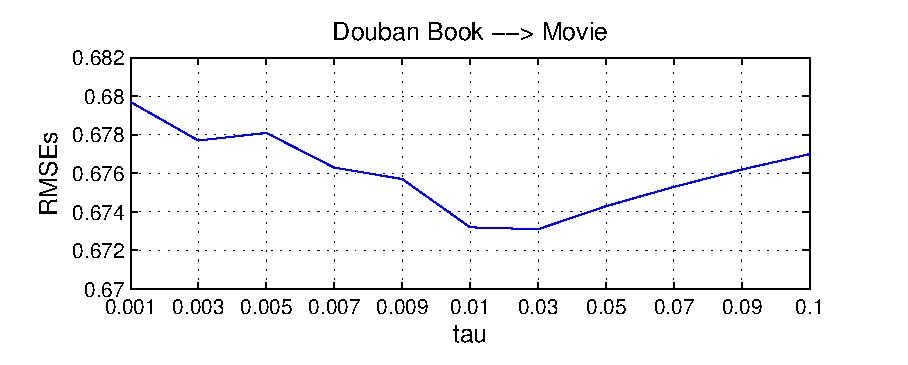
\includegraphics[width=6.5in]{fig/douban_tau.eps}
\caption{Change of the RMSEs with different $\tau$s. (Douban book to Movie)}\label{fig:tau1}
\end{figure}


\begin{figure}[t]
\centering
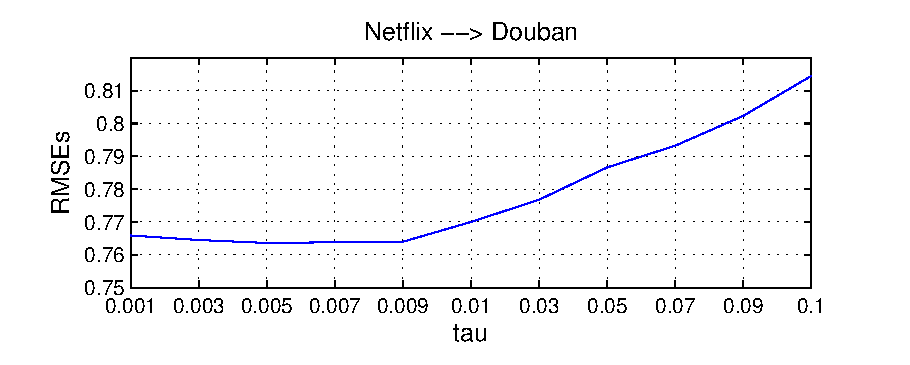
\includegraphics[width=6.5in]{fig/nf_tau.eps}
\caption{Change of the RMSEs with different $\tau$s. (Netflix to Douban Movie)}\label{fig:tau2}
\end{figure}


\begin{figure}[t]
\centering
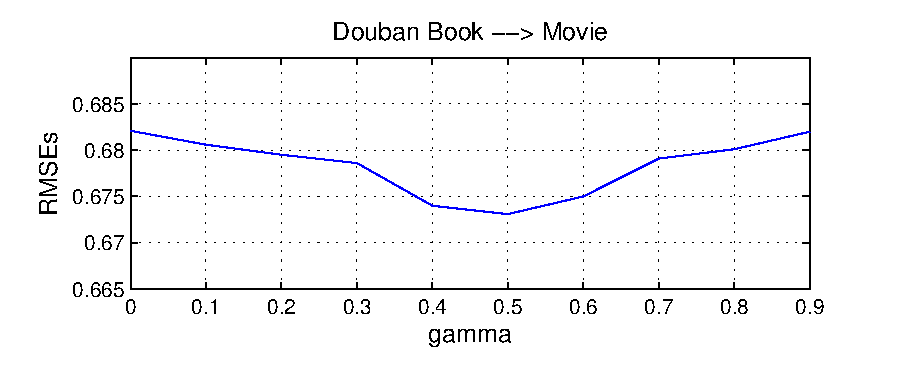
\includegraphics[width=6.5in]{fig/douban_gamma.eps}
\caption{Change of the RMSEs with different $\gamma$s. (Douban book to Movie)}\label{fig:gamma1}
\end{figure}


\begin{figure}[t]
\centering
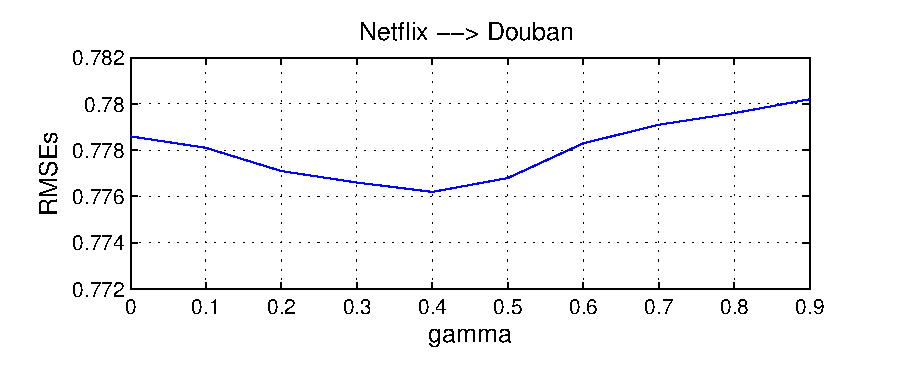
\includegraphics[width=6.5in]{fig/nf_gamma.eps}
\caption{Change of the RMSEs with different $\gamma$s. (Netflix to Douban Movie)}\label{fig:gamma2}
\end{figure}

\subsection{Convergence and Overfitting Test}
Figure \ref{fig:converge1} shows the RMSEs of STLCF(EV) as the number of weak learners changes on the Douban Book to Movie task. From the figure, we observe that STLCF(EV) converges well after 40 iterations. In Figure \ref{fig:converge2}, we can find that the corresponding $\alpha$ also converge to around 0.68 after 40 iterations as well. Empirically, we find STLCF converges in less than $50$ iterations.


\begin{figure}[t]
\centering
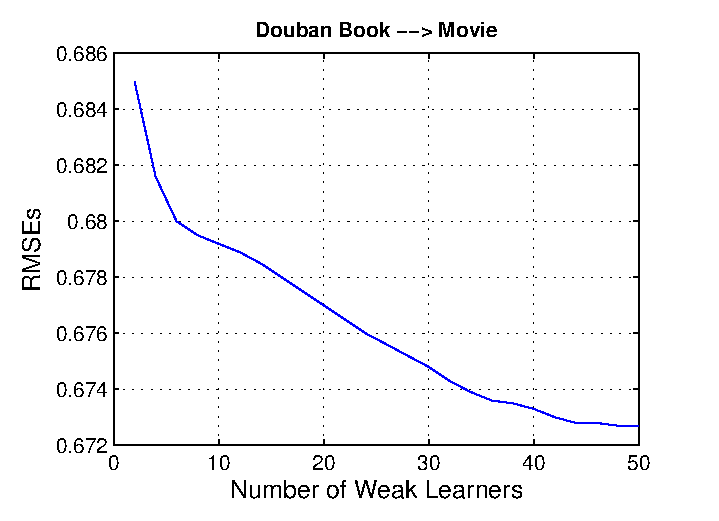
\includegraphics[width=6in]{fig/douban_learners.eps}
\caption{Change of the RMSEs when more and more weak learners join in the committee.}\label{fig:converge1}
\end{figure}

\begin{figure}[t]
\centering
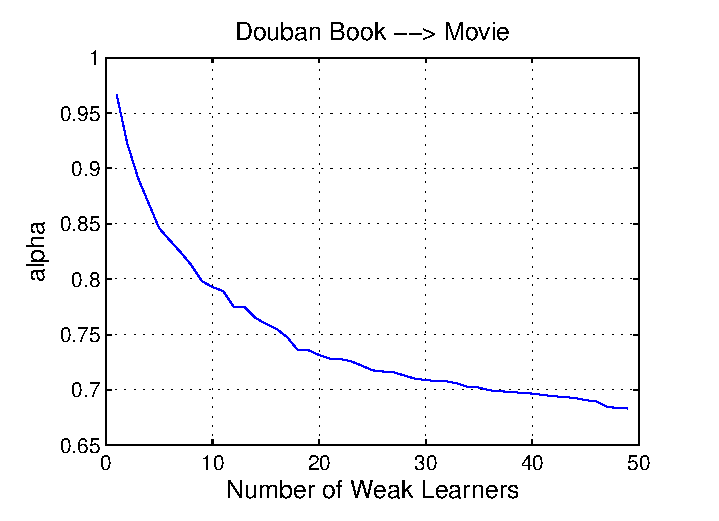
\includegraphics[width=6in]{fig/douban_alpha.eps}
\caption{Change of $\alpha$s when more and more weak learners join in the committee.}\label{fig:converge2}
\end{figure}

The number of latent topics of the base learner TGPLSA reflects the model's ability to fit training data. When we keep increasing the number of latent topics, the model tends to better fit the training data. But if the number of latent topics is too large, the model may suffer from overfitting.

We investigate the overfitting issue by plotting the training and testing RMSEs of the non-transfer learning model GPLSA, the non-selective transfer learning model TGPLSA and our selective transfer learning model STLCF(EV) over different numbers of latent topics in Figure \ref{fig:k}. The data sparsity for the target domain is around 0.3\%.

We can observe that comparing to our STLCF, the training RMSEs of GPLSA and TGPLSA decrease faster, while their testing RMSEs go down slower. When $k$ is about $50$, the testing RMSEs of GPLSA start to go up. And for TGPLSA, its testing RMSEs also go up slightly when $k$ is larger than $75$. But the testing RMSEs of our STLCF keep decreasing until $k=125$ and even when $k$ is larger than $125$, the raise of our STLCF's testing RMSEs is not obvious. Clearly when the target domain is very sparse, our STLCF method is more robust against the overfitting, by inheriting the advantage from boosting techniques and the fine-grained selection on knowledge transfer.

\begin{figure}
\begin{minipage}[t]{0.95\linewidth}
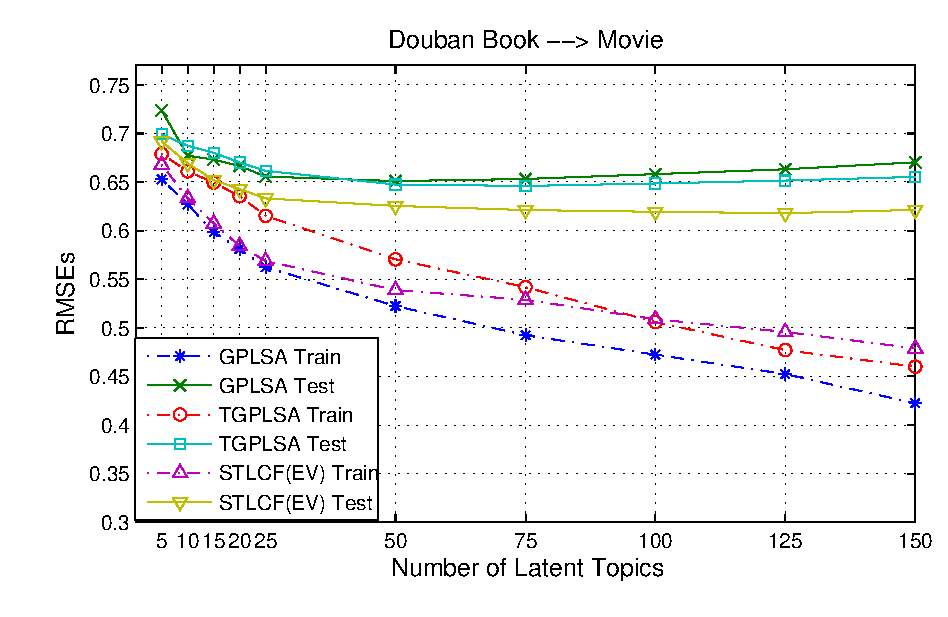
\includegraphics[width=6.5in]{fig/douban_k.eps}
\end{minipage}
\caption{Change of the RMSEs with different numbers of latent topics.}\label{fig:k}
\end{figure}

\chapter{Conclusion and Future work}
\label{chp:conclusion}

In this thesis, we proposed to perform knowledge transfer for one-class CF problems using matrix factorization and came up with a matrix tri-factorization method and a online framework to systematically study on the factors that will affect selection.
We found although there exists some methods which tackle the one-class CF problem and there are also some transfer learning methods for CF. But no one has deal with one-class CF in multiple domains. Simply apply former transfer learning methods will fail due to data sparsity. 
We found under matrix tri-factorization framework(TRIMF), we can transfer as much knowledge as we can while ignore the noise. 
By leveraging overlapped users and items, we can transfer knowledge from different domains. While applying the linear control factor to pattern matrix, we can avoid direct transfer which can bring noise while capture the similarity between different domains.
To put our method in reality, we developed a clustering based matrix factorization framework(CBMF) which automatically integrate all data together then perform matrix factorization.
The experimental results for TRIMF in real-word data sets showed that our method performs better than several state-of-the-art methods in conversion rate comparison.
The experimental results for CBMF in real-word showed that our method has the best conversion rate and moderate click through rate among others.
 
However, we notice that there are limitations in the work. First, in TRIMF, the computational cost is expensive since multiplicative rules will affect all matrix in update time. Second, we only support non-negative matrix factorization in TRIMF, because we need to constrain non-negative to fulfill optimization conditions. If matrix can be negative, it'll be more flexible and can carry more information. Third, both TRIMF and CBMF are point-wise methods which optimize for each entry of the matrix, actually we only need to rank those items not to calculate their score. That is, we only need their relative relationship \cite{Rendle:2009:BBP:1795114.1795167}. Fourth, TRIMF and CBMF are batch updated algorithms, but in online test almost all algorithms whose performance are good are real-time.


We believe that Transfer Learning for One-Class Recommendation has practical applications in the real world and would be a promising research topic. TRIMF/CBMF is our initial attempt on this topic. In the future to make it more robust, we propose the following approaches:
\begin{itemize}
\item {\bf Pair-wise Transfer Learning in CF.} Instead of point-wise transfer in CF, pair-wise CF is becoming more and more popular because they can almost achieve better results. In \cite{DBLP:dblp_conf/recsys/LercheJ14, DBLP:dblp_conf/recsys/Aiolli14} pair-wise CF is applied in implicit feedback. In transfer learning, integrating matrix factorization and pair-wise CF can be the future work.
\item {\bf Online Transfer Learning in CF.} There are little work on large scale transfer learning, but it is badly desirable. In real-world, online recommendation algorithms often dominant off-line ones. Our method CBMF is a batch-updating algorithm which updates per hour, but not real-time. It would be our future work to make a real online transfer learning algorithm in CF.
\item {\bf Transfer Learning in CF with multiple matrix.} In CBMF, data from different sources are integrated into one unify matrix. Although very carefully, we can still lose or misuse the data. If we can run our algorithm fast on their original data, then we don't need to integrate.
\item {\bf Time Complexity Optimization in CF.} In \cite{Shalev-Shwartz:2008:SOI:1390156.1390273}, an interesting relationship is shown: more data can faster training speed while getting the same performance on test data. In CF there are many data that we need plenty of time to deal with. If we could leverage all of them without increasing our training time or model complexity, we could use as much data as possible.
\end{itemize} 


%%%%%%%%%%%%%%%%%%%%%%%%%%%%%%%%%%%%%%%%%%%%%%%%%%%%%%%%%%%%%%%%%%%%%%%%%
%                                                                       %
% An example of a figure. Note how the Figure Number is generated in    %
% the list of figures.                                                  %
%                                                                       %
%%%%%%%%%%%%%%%%%%%%%%%%%%%%%%%%%%%%%%%%%%%%%%%%%%%%%%%%%%%%%%%%%%%%%%%%%



%%%%%%%%%%%%%%%%%%%%%%%%%%%%%%%%%%%%%%%%%%%%%%%%%%%%%%%%%%%%%%%%%%%%%%%%%
%                                                                       %
% An example of a table. Note how the Table Number is generated in the  %
% list of tables.                                                       %
%                                                                       %
%%%%%%%%%%%%%%%%%%%%%%%%%%%%%%%%%%%%%%%%%%%%%%%%%%%%%%%%%%%%%%%%%%%%%%%%%


%%%%%%%%%%%%%%%%%%%%%%%%%%%%%%%%%%%%%%%%%%%%%%%%%%%%%%%%%%%%%%%%%%%%%%%%%
%                                                                       %
%      9) BIBLIOGRAPHY                                                  %
%                                                                       %
% This example uses bibtex to generate the required Bibliography. Refer %
% to the % the file ustthesis_test.bib for the entries of the           %
% Bibliography. Note that only the cited entries are printed.           %
%                                                                       %
% If BibTeX is not used to typeset the bibliography, replace the        %
% following line with the \begin{thebibliography} and \end{bibliography}%
% commands (the "thebibliography" environment) to process the           %
% Bibliography.                                                         %
%                                                                       %
%%%%%%%%%%%%%%%%%%%%%%%%%%%%%%%%%%%%%%%%%%%%%%%%%%%%%%%%%%%%%%%%%%%%%%%%%

%%%%%%%%%%%%%%%%%%%%%%%%%%%%%%%%%%%%%%%%%%%%%%%%%%%%%%%%%%%%%%%%%%%%%%%%%
%                                                                       %
% The recommended bibliography style is the IEEE bibliography style.    %
% "ustbib" defines the IEEE bibliography standard with the added        %
% ability of sorting the items by name of author.                       %
%                                                                       %
% If you are not using BibTeX to process your Bibliography, comment out %
% the following line.                                                   %
%                                                                       %
%%%%%%%%%%%%%%%%%%%%%%%%%%%%%%%%%%%%%%%%%%%%%%%%%%%%%%%%%%%%%%%%%%%%%%%%%
%when you want to add the references, please release the following two lines:
\bibliographystyle{plain}
\bibliography{reference}
% Please run "bibtex ustthesis_test" before the bibliography can be
% included.

%%%%%%%%%%%%%%%%%%%%%%%%%%%%%%%%%%%%%%%%%%%%%%%%%%%%%%%%%%%%%%%%%%%%%%%%%
%                                                                       %
%     10) APPENDIX (If Any)                                              %
%                                                                       %
% \appendix command marks the beginning of the APPENDIX part of the     %
% Thesis. The usual \chapter command is used for the different chapters %
% of the Appendix.                                                      %
%                                                                       %
%%%%%%%%%%%%%%%%%%%%%%%%%%%%%%%%%%%%%%%%%%%%%%%%%%%%%%%%%%%%%%%%%%%%%%%%%

%%\appendix
%%\chapter{Proof of P=NP}
%%\begin{figure}[h]
%%\caption{Illustration of Turing's Modification}
%%\end{figure}
%%\chapter{Refutation of Church-Turing Thesis}

%%%%%%%%%%%%%%%%%%%%%%%%%%%%%%%%%%%%%%%%%%%%%%%%%%%%%%%%%%%%%%%%%%%%%%%%%
%                                                                       %
%     11) BIOGRAPHY (Optional)                                          %
%                                                                       %
% \biography and \endbiography are used to define the optional          %
% Biography of the author of the Thesis.                                %
%                                                                       %
%%%%%%%%%%%%%%%%%%%%%%%%%%%%%%%%%%%%%%%%%%%%%%%%%%%%%%%%%%%%%%%%%%%%%%%%%

%\biography
% The biography of the student is ALSO optional.
%\bibliography{Publications}
%\input{Publications}
%\endbiography

\end{document}

